\documentclass{beamer}
\usetheme{Madrid}
\usepackage{array}
\setbeamertemplate{caption}[numbered]
\title[CST 309 M2]{MANAGEMENT OF SOFTWARE SYSTEMS}
\subtitle{Module 2}
\author{Rijin IK}
\institute[VJEC]{Assistant Professor\\Department of Computer Science and Engineering\\Vimal Jyothi Engineering College\\Chemperi}
\begin{document}
	\begin{frame}
		\titlepage
	\end{frame}
   \begin{frame}{Outline}
   \tableofcontents
   \end{frame}
\section{Functional and non-functional requirements}
\begin{frame}{Functional and non-functional requirements}
\textbf{Requirements}
\begin{itemize}
	\item The descriptions of the services that a system 
	should provide and the constraints on its operation.
\end{itemize}
\textbf{Requirements Engineering (RE)}
\begin{itemize}
	\item The process of finding out, analyzing, documenting and checking the services 
	and constraints of a system.
	\item The first stage of the software engineering process.
\end{itemize}
\end{frame}
\begin{frame}{Functional and non-functional requirements}
	
\textbf{Concept of User and System Requirements}
\begin{itemize}
	\item 	\textbf{User requirements }
	\begin{itemize}
		\item User requirements are statements, in a natural language plus diagrams, of what services the system is expected to provide to system users and the constraints under which it must operate. 
		\item High-level abstract requirements.
	\end{itemize}
	\item \textbf{System requirements}
	\begin{itemize}
		\item Detailed description of what the 
		system should do.
		\begin{itemize}
			\item Detailed descriptions of the software 
			system’s functions, services, and 
			operational constraints.
		\end{itemize}
		\item The system requirements document (sometimes called a functional specification) should define exactly what is to be implemented. 
	\end{itemize}
\end{itemize}
\end{frame}
\begin{frame}{Functional and non-functional requirements}
		\begin{figure}
		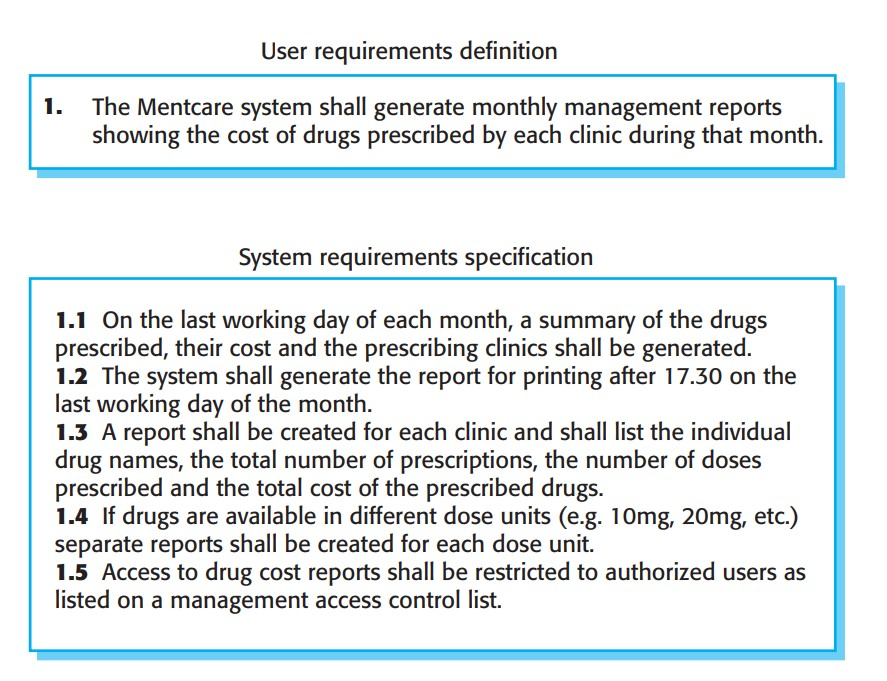
\includegraphics[scale=.5]{img/m2_1.jpg}
		\caption{User and 
			system requirements}
	\end{figure}
\end{frame}
\begin{frame}{Functional and non-functional requirements}
	\begin{center}
		\begin{tabular}{| p{5cm} | p{5cm} |}
			\hline
			\textbf{Functional Requirements} & \textbf{Non-functional Requirements}  \\ 
			\hline
			\begin{itemize}
				\item Statements of services the 
				system should provide
				\item How the 
				system should react to particular 
				inputs
				\item How the system 
				should behave in particular 
				situations.
			\end{itemize}
	 &  Constraints on the services or 
			functions offered by the system.
 \\  
			\hline
		 Explicitly state what the system 
		should not do. & Include timing constraints, 
		constraints on the development 
		process, and constraints 
		imposed by standards. \\
			\hline
		\end{tabular}
	\end{center}
\end{frame}
\begin{frame}{Functional and non-functional requirements}
\textbf{Functional Requirements}
\begin{itemize}
	\item Describe what the system should do.
	\item Describe functionality or system services
	\item These 
	requirements depends on the type of software being developed, the expected 
	users of the software, and the general approach taken by the 
	organization when writing requirements.
	\item When expressed as user requirements, it should be written in natural 
	language so that system users and managers can understand them.
	\item Functional system 
	requirements expand the user requirements and are written for system developers. 
	\item The user and system requirements should 
	be clear, unambiguous, easy to understand, complete, and consistent.

\end{itemize}
\end{frame}
\begin{frame}{Functional and non-functional requirements}
	\textbf{Examples for functional requirements for the Mentcare
		system:}
	\begin{enumerate}
		\item A user shall be able to search the appointments lists for all clinics.
		\item The system shall generate each day, for each clinic, a list of patients 
		who are expected to attend appointments that day.
		\item Each staff member using the system shall be uniquely identified by 
		his or her eight-digit employee number.
	\end{enumerate}
\end{frame}
\begin{frame}{Functional and non-functional requirements}
	\textbf{Non- functional Requirements}
	\begin{itemize}
		\item Non-Functional Requirements defines the constraints or characteristics on the system.
		\item Non-Functional Requirements deal with issues like scalability, maintainability, performance, portability, security, reliability, and many more.
		\item Failing to meet a non-functional requirement can mean that the whole system is 
		unusable.
	
		\item The implementation of these requirements may be spread throughout the system, for two reasons
		\begin{enumerate}
			\item May affect the overall architecture of a system rather than the individual components.
			\item May generate several, related functional requirements that define new system services 
			that are required if the non-functional requirement is to be implemented.
		\end{enumerate}
	\end{itemize}
\end{frame}

\begin{frame}{Functional and non-functional requirements}
	\textbf{Types of nonfunctional requirement}
\begin{enumerate}
	\item \textbf{Product requirements }
	\begin{itemize}
		\item These requirements specify or constrain the runtime 
		behavior of the software.
		\item Examples include how fast the system must execute, how much memory 
		it requires, etc
	\end{itemize}
	\item \textbf{Organizational requirements}
	\begin{itemize}
		\item These requirements are broad system requirements derived from policies and procedures in the customer’s and developer’s 
		organizations.
		\item e.g. Process 
		standards used, implementation requirements, etc.
	\end{itemize}
\item \textbf{External requirements}
\begin{itemize}
	\item This broad heading covers all requirements that are 
	derived from factors external to the system and its development process.
	\item e.g. interoperability requirements, legislative 
	requirements, etc 
\end{itemize}
\end{enumerate}
\end{frame}
\begin{frame}{Functional and non-functional requirements}
	\textbf{Types of nonfunctional requirement}
	\begin{figure}
		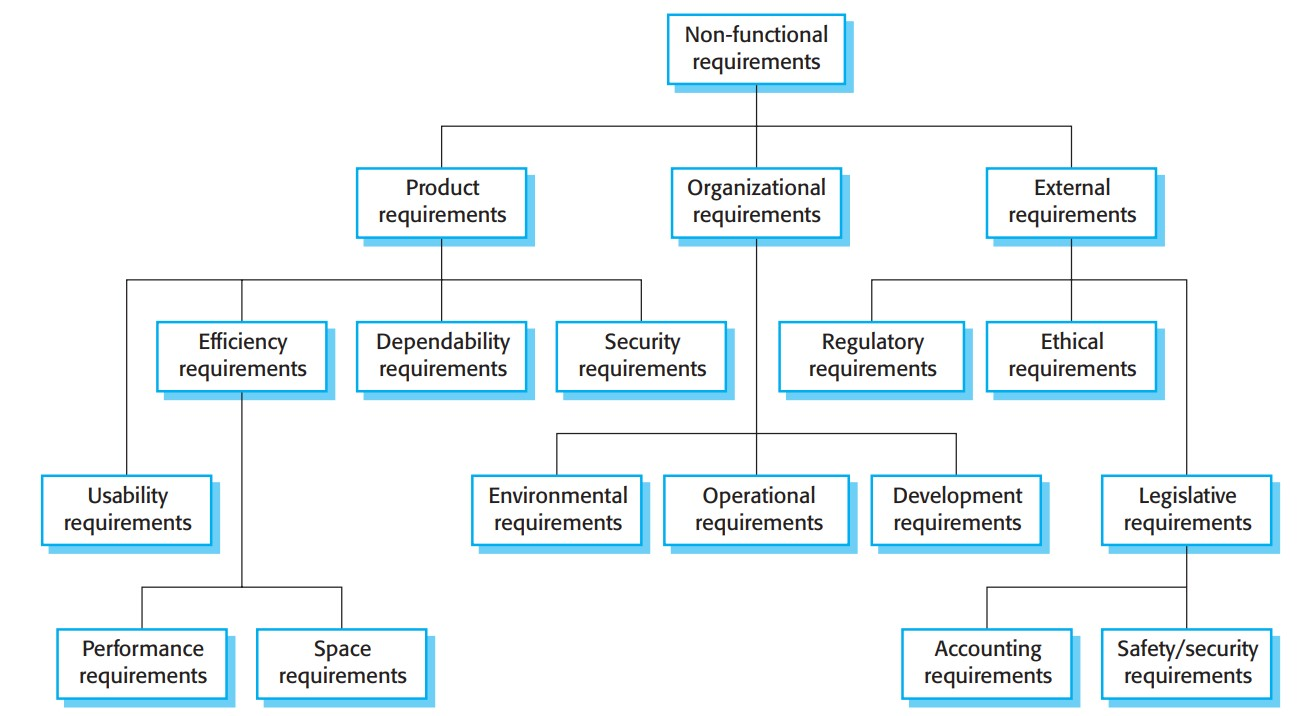
\includegraphics[scale=.4]{img/m2_2.jpg}
		\caption{Types of non-functional requirements}
	\end{figure}
\end{frame}
\begin{frame}{Functional and non-functional requirements}
	\textbf{Examples of 
		possible non-functional 
		requirements for the 
		Mentcare system}
		\begin{figure}
		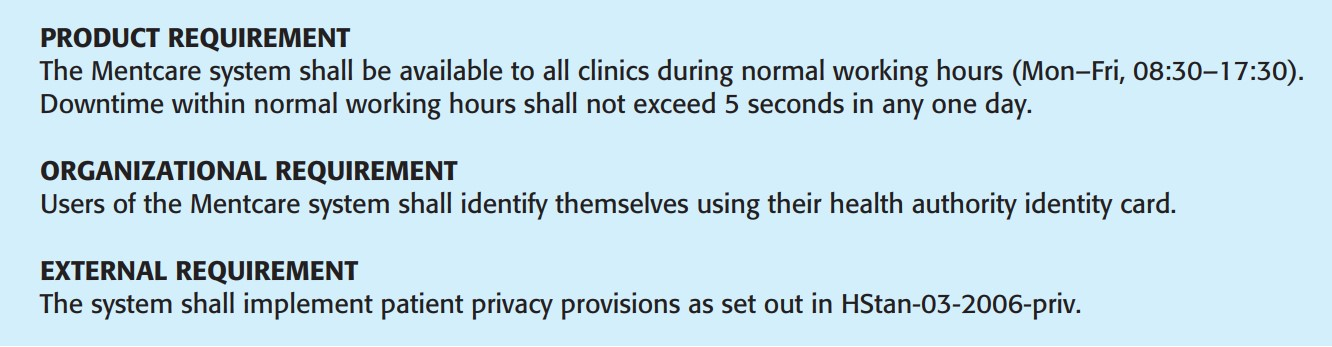
\includegraphics[scale=.4]{img/m2_3.jpg}
	\end{figure}

\end{frame}
\begin{frame}{Functional and non-functional requirements}
	\textbf{ Metrics for specifying non-functional requirements}
	\begin{figure}
		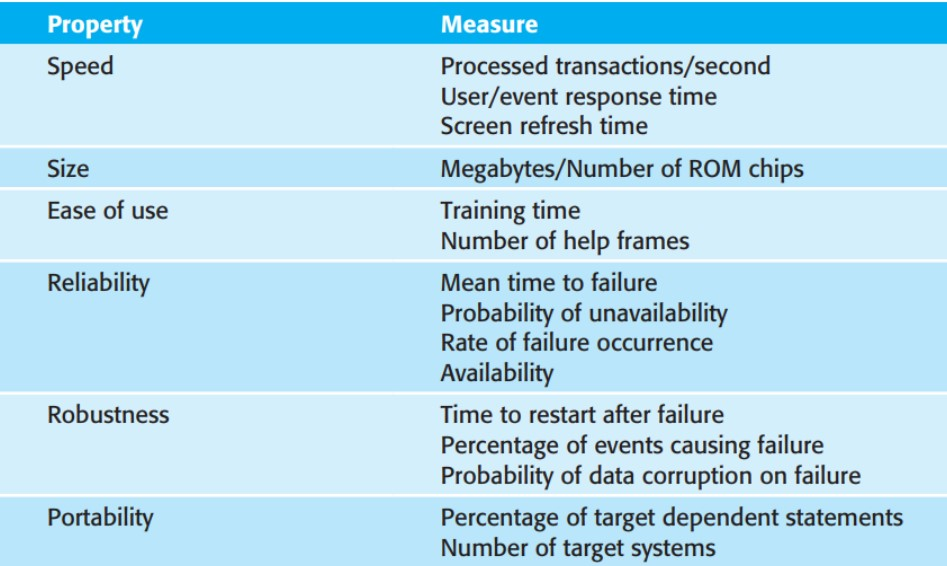
\includegraphics[scale=.5]{img/m2_4.jpg}
	\end{figure}
	
\end{frame}
\section{Requirements engineering processes}
\begin{frame}{Requirements engineering processes}
	\textbf{Requirements engineering processes}
	\begin{itemize}
		\item The process of finding out, analyzing, documenting and checking the services 
		and constraints of a system.
	\end{itemize}
RE involves three key activities:
\begin{enumerate}
	\item Discovering requirements by interacting with stakeholders (elicitation and analysis)
	\item Converting these requirements into a standard form (specification)
	\item Checking that the requirements actually define the system that the 
	customer wants (validation)
\end{enumerate}
The output of the RE process is a system requirements document.
\end{frame}
\begin{frame}{Requirements engineering processes}
	
	\begin{figure}
	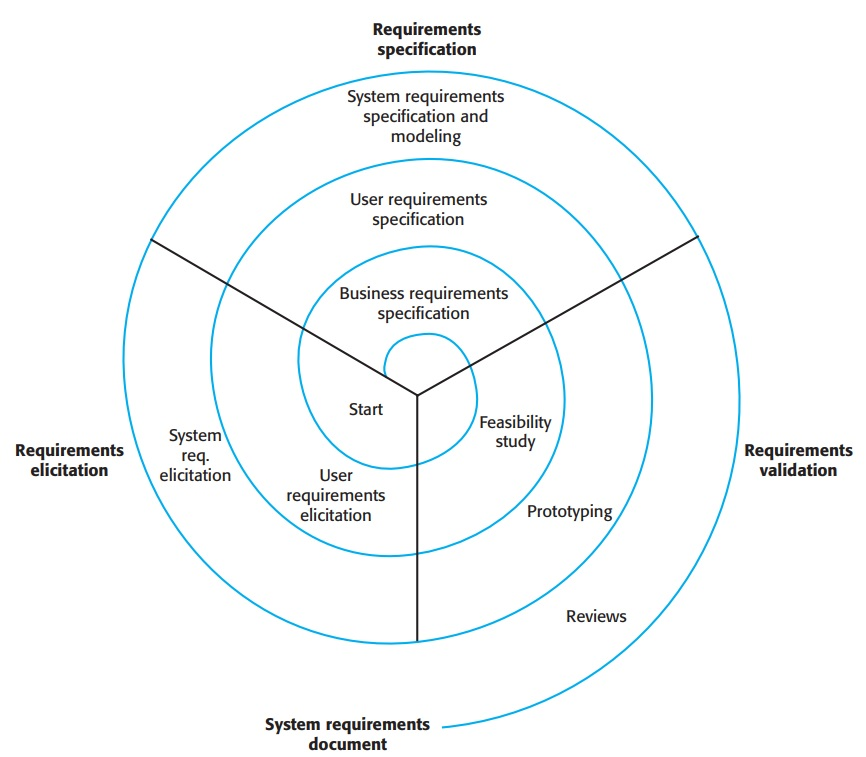
\includegraphics[scale=.45]{img/m2_5.jpg}
	\caption{A spiral view 
		of the requirements 
		engineering process}
\end{figure}
\end{frame}
\section{Requirements elicitation}
\begin{frame}{Requirements elicitation}
	\textbf{Requirements elicitation}
	\begin{itemize}
		\item The aims of the requirements elicitation process are to understand the work that stakeholders   do and how they might use a new system to help support that work.
		\item During requirements elicitation, software engineers work with stakeholders to find out about    the application domain, work activities, the services and system features that stakeholders want, the required performance of the system, hardware constraints, and so on.
		
	\end{itemize}
\end{frame}
\begin{frame}{Requirements elicitation}
	\textbf{Difficulties/challenges in Eliciting and understanding requirements}
	\begin{itemize}
		\item Stakeholders often don’t know what they want from a computer system 
		except in the most general terms.
		\item Stakeholders in a system naturally express requirements in their own terms 
		and with implicit knowledge of their own work.
		\item Different stakeholders, with diverse requirements, may express their 
		requirements in different ways.
		\item Political factors may influence the requirements of a system. 
		\item The economic and business environment in which the analysis takes place 
		is dynamic. New requirements may emerge from new stakeholders who 
		were not originally consulted.
	\end{itemize}
\end{frame}
\begin{frame}{Requirements elicitation}
	\textbf{The requirements elicitation and analysis process }
	\begin{figure}
		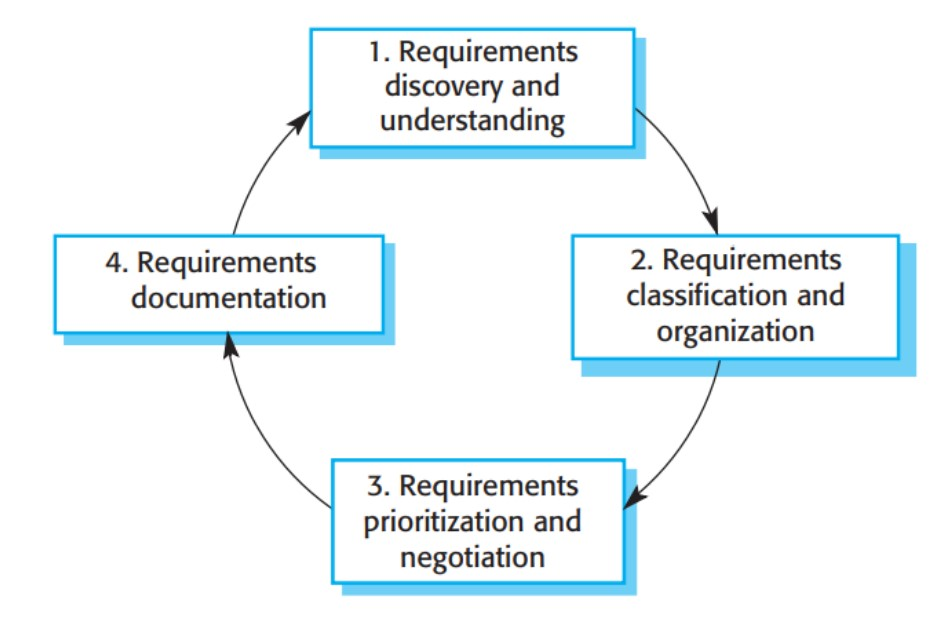
\includegraphics[scale=.45]{img/m2_6.jpg}
		\caption{The requirements elicitation and analysis process}
	\end{figure}
\end{frame}
\begin{frame}{The requirements elicitation and analysis process }
	\textbf{Requirements discovery and understanding }
	\begin{itemize}
		\item This is the process of interacting with stakeholders of the system to discover their requirements. Domain requirements from stakeholders and documentation are also discovered during this activity.
	\end{itemize}
\textbf{Requirements classification and organization }
\begin{itemize}
	\item This activity takes the unstructured collection of requirements, groups related requirements and organizes them into coherent clusters.
\end{itemize}
\textbf{Requirements prioritization and negotiation }
\begin{itemize}

	\item This activity is concerned with prioritizing requirements and finding and resolving requirements conflicts through negotiation(when multiple stakeholders are involved). Usually, stakeholders have to meet to resolve differences and agree on compromise requirements.
\end{itemize}
\textbf{Requirements documentation }
\begin{itemize}
	\item The requirements are documented and input into the next round of the spiral. An early draft of the software requirements documents may be produced at this stage.
\end{itemize}
\end{frame}
\begin{frame}{Requirements elicitation}
	\textbf{Requirements elicitation techniques}\\
	There are two fundamental approaches to requirements elicitation:
	\begin{enumerate}
		\item \textbf{Interviewing}, where you talk to people about what they do.
		\item \textbf{Observation or ethnography}, where you watch people doing their job to see what artifacts     they use, how they use them, and so on.
	\end{enumerate}
\end{frame}
\begin{frame}{Requirements elicitation techniques}
	\textbf{Interviewing}\\
	Interviews may be of two types:
	\begin{itemize}
		\item \textbf{Closed interviews}, where the stakeholder answers a predefined set of questions.
		\item \textbf{Open interviews}, in which there is no predefined agenda. The requirements engineering team explores a range of issues with system stakeholders and hence develops a better understanding of their needs.
	\end{itemize}
To be an effective interviewer, you should bear two things in mind
\begin{itemize}
	\item You should be open-minded, avoid preconceived ideas about the requirements, 
	and willing to listen to stakeholders.
	\item You should prompt the interviewee to get discussions going by using a springboard 
	question or a requirements proposal, or by working together on a prototype 
	system.
\end{itemize}
\end{frame}
\begin{frame}{Requirements elicitation techniques}
	\textbf{Ethnography}
	\begin{itemize}
		\item The day-to-day work is observed, and notes are made of the actual tasks in which participants  are involved. 
		\item The value of ethnography is that it helps discover implicit system requirements that reflect the actual ways that people work, rather than the formal processes defined by the organization.
	\end{itemize}
Ethnography is particularly effective for discovering two types of requirements:
\begin{enumerate}
	\item Requirements derived from the way in which people actually work, rather than the way in which business process definitions say they ought to work. In practice, people never    follow formal processes. 
	
	\item Requirements derived from cooperation and awareness of other people’s activities.
	
\end{enumerate}
\end{frame}
\begin{frame}{Requirements elicitation techniques}
\begin{figure}
	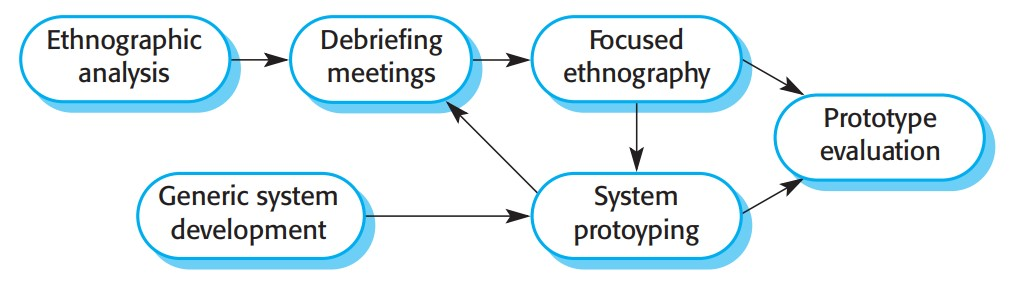
\includegraphics[scale=.45]{img/m2_7.jpg}
	\caption{Ethnography 
		and prototyping for 
		requirements analysis}
\end{figure}

\end{frame}


\section{Requirements validation}
\begin{frame}{Requirements validation}
	\textbf{Requirements validation}
	\begin{itemize}
		\item Requirements validation is the process of checking that requirements define the system      that the customer really wants.
		\item Requirements validation is critically important because errors in a requirements document  can lead to extensive rework costs when these problems are discovered during development or after the system is in service.
	\end{itemize}
\end{frame}
\begin{frame}{Requirements validation}
	During the requirements validation process, different types of checks should be carried out on  the requirements in the requirements document. These checks include:
	\begin{enumerate}
		\item \textbf{Validity checks} check that the requirements reflect the real needs of system users.
		\item \textbf{Consistency checks} requirements in the document should not conflict. 
		\item \textbf{Completeness checks} requirements document should include requirements that define all functions and the constraints intended by the	system user.

		\item \textbf{Realism checks} checked to ensure that they can be implemented within the proposed budget for the system.
		\item \textbf{Verifiability} system requirements should always be written so that they are verifiable.
		
	\end{enumerate}
\end{frame}
\begin{frame}{Requirements validation}
\textbf{Requirements validation techniques }
\begin{enumerate}
	\item \textbf{Requirements reviews} The requirements are analyzed systematically by a team of reviewers who check for errors and inconsistencies.
	\item \textbf{Prototyping:} 
		This involves developing an executable model of a system and using this with end-users and customers to see if it meets their needs and expectations. Stakeholders experiment with the system and feed back requirements changes to the development team.
	\item \textbf{Test-case generation:} 
		Requirements should be testable. If a test is difficult or impossible to design, this usually means that the requirements will be difficult to implement and should be reconsidered. Developing tests from the user requirements before any code is written is an integral part of test-driven development.
\end{enumerate}
\end{frame}
\section{Requirements change}
\begin{frame}{Requirements change}
	\textbf{Requirements change}
	\begin{enumerate}
		\item Requirements management planning
		\item Requirements change management
	\end{enumerate}
\end{frame}

\begin{frame}{Requirements change}
	\textbf{Requirements change}
	\begin{itemize}
		\item The requirements for large software systems are always changing. One reason for the frequent changes is that these systems are often developed to address “wicked” problems—problems that cannot be completely defined. 
	\end{itemize}
\begin{figure}
	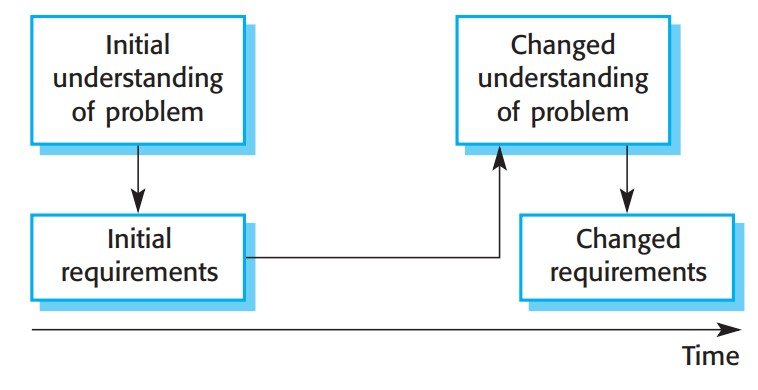
\includegraphics[scale=.45]{img/m2_8.jpg}
	\caption{Requirements evolution}
\end{figure}
\end{frame}
\begin{frame}{Requirements change}
	\textbf{Reason}\\
	 Most changes to system requirements arise because of changes to 
	the business environment of the system
	\begin{itemize}
		\item The business and technical environment of the system always changes after installation. New hardware may be introduced and existing hardware updated. 
	\item The people who pay for a system and the users of that system are rarely the same people.
	\begin{itemize}
		\item System customers impose requirements because of organizational and budgetary constraints. These may conflict with end-user requirements, and, after delivery, new features may have to be added for user support if the system is to meet its goals.
	\end{itemize}  
	\item Large systems usually have a diverse stakeholder community, with stakeholders having different requirements. Their priorities may be conflicting or contradictory. 	
	\end{itemize}
\end{frame}
\begin{frame}{Requirements change}
	\textbf{ Requirements management planning}
\begin{itemize}
	\item Requirements management planning is concerned with establishing how a set of evolving requirements will be managed. 
	\item During the planning stage, you have to 
	decide on a number of issues:
	\item \textbf{Requirements management decisions:}
	\begin{itemize}
		\item \textbf{Requirements identification:} Each requirement must be uniquely identified so that it can 
		be cross-referenced with other requirements. 
		\item \textbf{A change management process:} This is the set of activities that assess the impact and 
		cost of changes.
		\item \textbf{Traceability policies:} These policies define the relationships between each requirement 
		and between the requirements and the system design that should be recorded. 
		\item \textbf{Tool support:}  Requirements management involves the processing of large 
		amounts of information about the requirements. Tools that may be used range 
		from specialist requirements management systems to shared spreadsheets and 
		simple database systems.

	\end{itemize}
\end{itemize}
\end{frame}
\begin{frame}{Requirements change}
	\textbf{Requirements change management}\\
	Deciding if a requirements change should be accepted
\begin{figure}
	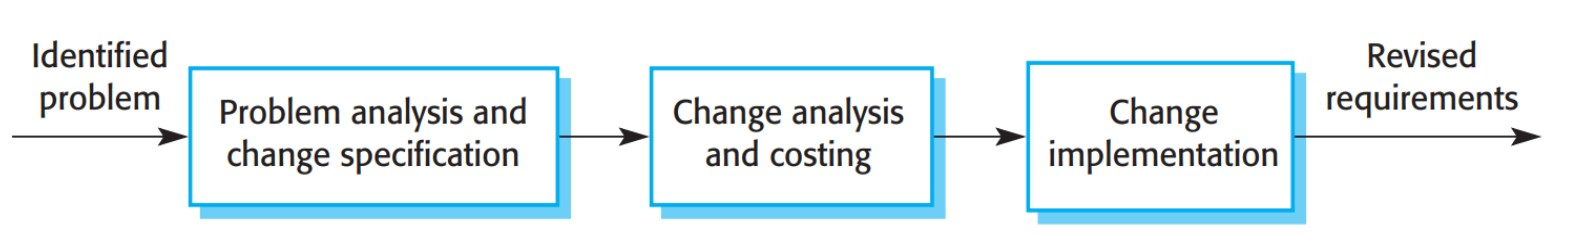
\includegraphics[scale=.34]{img/m2_9.jpg}
	\caption{Requirements change management}
\end{figure}
\end{frame}
\begin{frame}{Requirements change management}
	\textbf{Problem analysis and change specification}
\begin{itemize}
	\item During this stage, the problem or the change proposal is analyzed to check that it is valid. 
	\item This analysis is fed back to the change requestor who may respond with a more specific 
	requirements change proposal, or decide to withdraw the request.
\end{itemize}
\textbf{Change analysis and costing}
\begin{itemize}
	\item The effect of the proposed change is assessed using traceability information and general 
	knowledge of the system requirements.
	\item  Once this analysis is completed, a decision is 
	made whether or not to proceed with the requirements change.

\end{itemize}
\textbf{Change implementation}
\begin{itemize}
	\item The requirements document and, where necessary, the system design and 
	implementation, are modified. Ideally, the document should be organized so that 
	changes can be easily implemented.
	
\end{itemize}
\end{frame}
\section{Traceability Matrix}
\begin{frame}{Traceability Matrix}
	\textbf{Traceability Matrix}
\begin{itemize}
	\item Traceability matrix is a table type document that is used in the development of software application to trace requirements.
	\item In this document the test cases are mapped to the corresponding requirement
	\begin{itemize}
		\item To ensure that every requirement is covered in the form of a test case
		\item To find any gap between requirement and test case
	\end{itemize} 
	\item It can be used for both forward (from Requirements to Design or Coding) and backward (from Coding to Requirements) tracing.
	\item It is also known as \textbf{Requirement Traceability Matrix (RTM)} or \textbf{Cross Reference Matrix (CRM)}. 

\end{itemize}
\end{frame}
\begin{frame}{Traceability Matrix}
\begin{figure}
	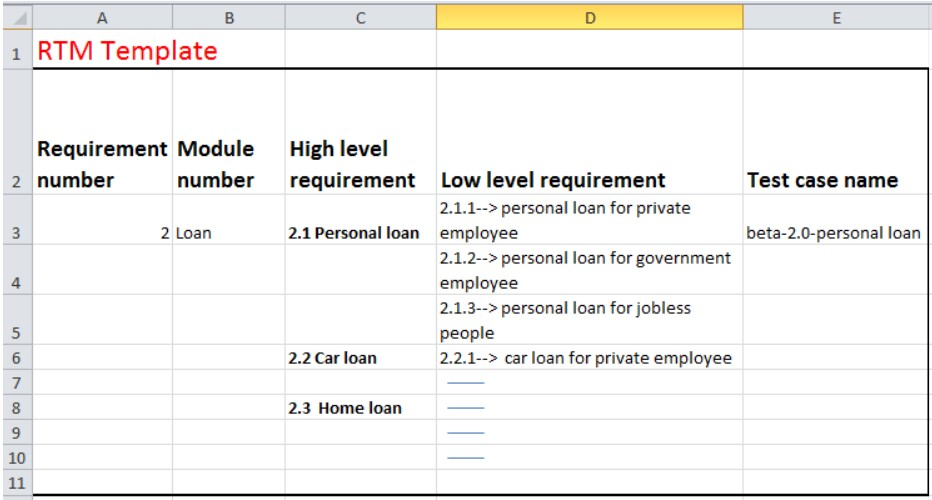
\includegraphics[scale=.55]{img/m2_12.jpg}
	\caption{Example of RTM template}
\end{figure}
\end{frame}
\begin{frame}{Traceability Matrix}
	\textbf{Goals of Traceability Matrix:}
	\begin{itemize}
		\item It helps in tracing the documents that are developed during various phases of SDLC.
		\item It ensures that the software completely meets the customer's requirements.
		\item It helps in detecting the root cause of any bug.
	\end{itemize}
	\textbf{Types of Traceability Test Matrix}\\
The traceability matrix can be classified into three different types which are as follows:
\begin{itemize}
	\item Forward traceability
	\item Backward or reverse traceability
	\item Bi-directional traceability
\end{itemize}
\end{frame}
\begin{frame}{Traceability Matrix}
	\textbf{Forward Traceability }
	\begin{itemize}
		\item The forward traceability test matrix is used to ensure that every business's needs or requirements are executed correctly in the application and also tested rigorously. 
		\item The main objective of this is to verify whether the product developments are going in the right direction. 
		\item In this, the requirements are mapped into the forward direction to the test cases.
	\end{itemize}
\begin{figure}
	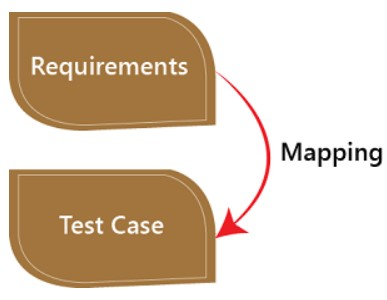
\includegraphics[scale=.5]{img/m2_13.jpg}
	\caption{Forward Traceability}
\end{figure}
\end{frame}
\begin{frame}{Traceability Matrix}
	\textbf{Backward or reverse traceability }
	\begin{itemize}
		\item The reverse or backward traceability is used to check that we are not increasing the space of the product by enhancing the design elements, code, test other things which are not mentioned in the business needs. 
		\item And the main objective of this that the existing project remains in the correct direction. 
		\item In this, the requirements are mapped into the backward direction to the test cases.
	\end{itemize}
	\begin{figure}
		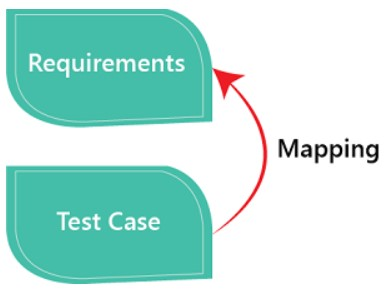
\includegraphics[scale=.5]{img/m2_14.jpg}
		\caption{Backward or reverse traceability}
	\end{figure}
\end{frame}
\begin{frame}{Traceability Matrix}
	\textbf{Bi-directional traceability }
	\begin{itemize}
		\item It is a combination of forwarding and backward traceability matrix, which is used to make sure that all the business needs are executed in the test cases.
		\item It also evaluates the modification in the requirement which is occurring due to the bugs in the application.
		
		
	\end{itemize}
	\begin{figure}
		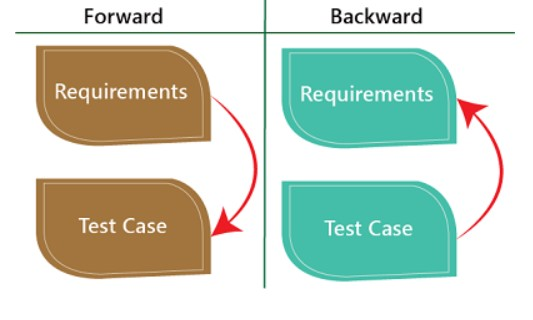
\includegraphics[scale=.5]{img/m2_15.jpg}
		\caption{Bi-directional traceability}
	\end{figure}
\end{frame}
\begin{frame}{Traceability Matrix}
	\textbf{Advantage of RTM }
	\begin{itemize}
		\item With the help of the RTM document, we can display the complete test execution and bugs status based on requirements.
		\item It is used to show the missing requirements or conflicts in documents.
		\item In this, we can ensure the complete test coverage, which means all the modules are tested.
		\item It will also consider the efforts of the testing teamwork towards reworking or reconsidering on the test cases.
	\end{itemize}
\end{frame}
\section{Developing use cases}
\begin{frame}{Developing use cases}
	\textbf{Use case}
\begin{itemize}
	\item Use case is , how an end user (playing one of a number of possible roles) interacts with the system under a specific set of circumstances. 
	\item It may be,
	\begin{itemize}
		\item A narrative text
		\item An outline of tasks or interactions.
		\item A template-based description.
		\item A diagrammatic representation. 
	\end{itemize}
\item Regardless of its form, a use case depicts the software or system from the end user’s point of view.
\end{itemize}
\end{frame}
\begin{frame}{Developing use cases}
	
\textbf{DEVELOPING USE CASES}
\begin{itemize}
	\item 	The first step in writing a use case is to define the set of \textbf{“actors”} that will be involved in the story.
   \item \textbf{Actor}
	\begin{itemize}
		\item The users that interact with a system. 
		\item An actor can be a person, an organization, or an outside system that interacts with your application or system.
		\item They must be external objects that produce or consume data.
	\end{itemize}
\item An actor and an end user are not necessarily the same thing.
\item A typical user may play a number of different roles when using a system, whereas an actor represents a class of external entities (often, but not always, people) that play just one role in the context of the use case. 
\end{itemize}
\end{frame}
\begin{frame}{Developing use cases}
	\textbf{Example}
	\begin{itemize}
		\item Consider a machine operator (a user) who interacts with the 
		control computer for a manufacturing cell that contains a number of 
		robots and numerically controlled machines.
		\item After careful review of requirements, the software for the control computer requires four different modes (roles) for interaction: 
		\begin{itemize}
			\item programming mode
			\item test mode
			\item monitoring mode
			\item troubleshooting mode. 
		\end{itemize}
	\item Therefore, four actors can be defined: programmer, tester, monitor, and troubleshooter. 
	\end{itemize}
\end{frame}
\begin{frame}{Developing use cases}
	\textbf{Types of actor}
\begin{itemize}
	\item Because requirements elicitation is an evolutionary activity, not all actors are identified   during the first iteration. 
	\item It is possible to identify \textbf{primary actors}  during the first iteration and \textbf{secondary actors} as more is learned about the system. 
\end{itemize}
\textbf{Primary actors }
\begin{itemize}
	\item Primary actors interact to achieve required system function and derive the intended benefit from the system. 
	\item They work directly and frequently with the software. 
\end{itemize}
\textbf{Secondary actors }
\begin{itemize}
	\item Secondary actors support the system so that primary actors can do their work.
\end{itemize}
Once actors have been identified, use cases can be developed
\end{frame}
\begin{frame}{Developing use cases}
\textbf{A number of questions should be answered by a use case}\\
\begin{enumerate}
	\item Who is the primary actor, the secondary actor(s)?
	\item What are the actor’s goals?
	\item What preconditions should exist before the story begins?
	\item What main tasks or functions are performed by the actor?
	\item What exceptions might be considered as the story is described?
	\item What variations in the actor’s interaction are possible?
	\item What system information will the actor acquire, produce, or change?
	\item Will the actor have to inform the system about changes in the external environment?
	\item What information does the actor desire from the system?
	\item Does the actor wish to be informed about unexpected changes?
	
\end{enumerate}
\end{frame}
\begin{frame}{Developing use cases}
	\textbf{Example:basic SafeHome requirements define 4 actors:}
	\begin{enumerate}
		\item homeowner (a user), 
		\item setup manager (likely the same person as homeowner, but playing a different role), 
		\item sensors (devices attached to the system), and 
		\item monitoring and response subsystem (the central station that monitors the SafeHome home security function). 
		
	\end{enumerate}
	For the purposes of this example, we consider only the homeowner actor. The 
	homeowner actor interacts with the home security function in a number of 
	different ways using either the alarm control panel or a PC. \\
		\textbf{The homeowner:}
	\begin{itemize}
		\item enters a password to allow all other interactions, 
		\item inquires about the status of a security zone, 
		\item inquires about the status of a sensor, 
		\item presses the panic button in an emergency, and 
		\item activates/deactivates the security system.
		
	\end{itemize}
\end{frame}
\begin{frame}{Developing use cases}
	\textbf{Considering the situation in which the homeowner uses the control panel, the
		basic use case for system activation follows:
	}
	\begin{itemize}
		\item[1] The homeowner observes the SafeHome control panel  to determine
		if the system is ready for input.
		\begin{itemize}
			\item If the system is not ready, a not ready message is
			displayed on the LCD display,
			\item and the homeowner must physically close windows
			or doors so that the not ready message disappears. [A not ready message implies
			that a sensor is open; i.e., that a door or window is open.]
		\end{itemize} 
		\item[2] The homeowner uses the keypad to key in a four-digit password.
		\begin{itemize}
			\item  The password is
			compared with the valid password stored in the system.
			\item If the password is incorrect,
			the control panel will beep once and reset itself for additional input.
			\item If the
			password is correct, the control panel awaits further action.
		\end{itemize}  
		
		
	\end{itemize}
	
\end{frame}
\begin{frame}{Developing use cases}
	\begin{itemize}
		\item[3] The homeowner selects and keys in stay or away  to activate the
		system. 
		\begin{itemize}
			\item Stay activates only perimeter sensors (inside motion detecting sensors are
			deactivated). Away activates all sensors.
		\end{itemize}
		\item[4] When activation occurs, a red alarm light can be observed by the homeowner.
	\end{itemize}
	
\end{frame}
\begin{frame}{Developing use cases}

	\begin{figure}
		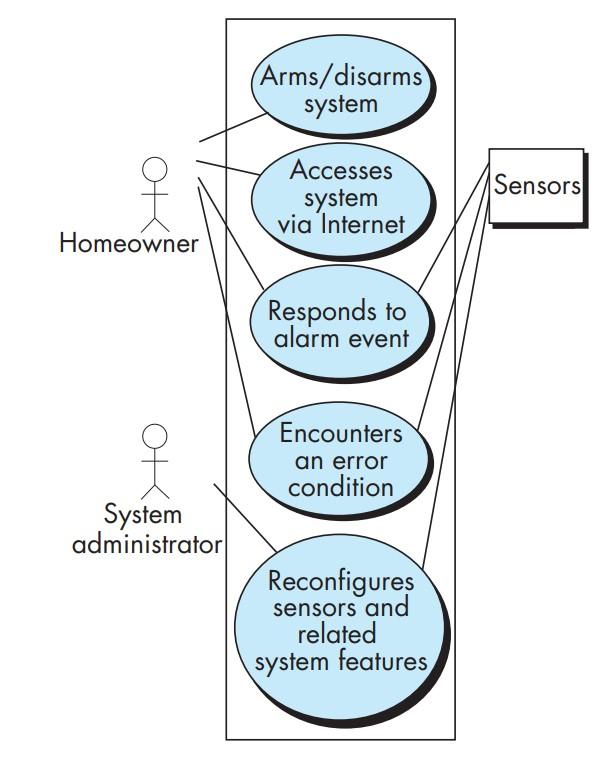
\includegraphics[scale=.4]{img/m2_16.jpg}
		\caption{use case 
			diagram for 
			SafeHome 
			home security 
			function }
	\end{figure}
\end{frame}
\begin{frame}{Developing use cases}
	\textbf{Template for detailed descriptions of use cases:}
		\begin{figure}
		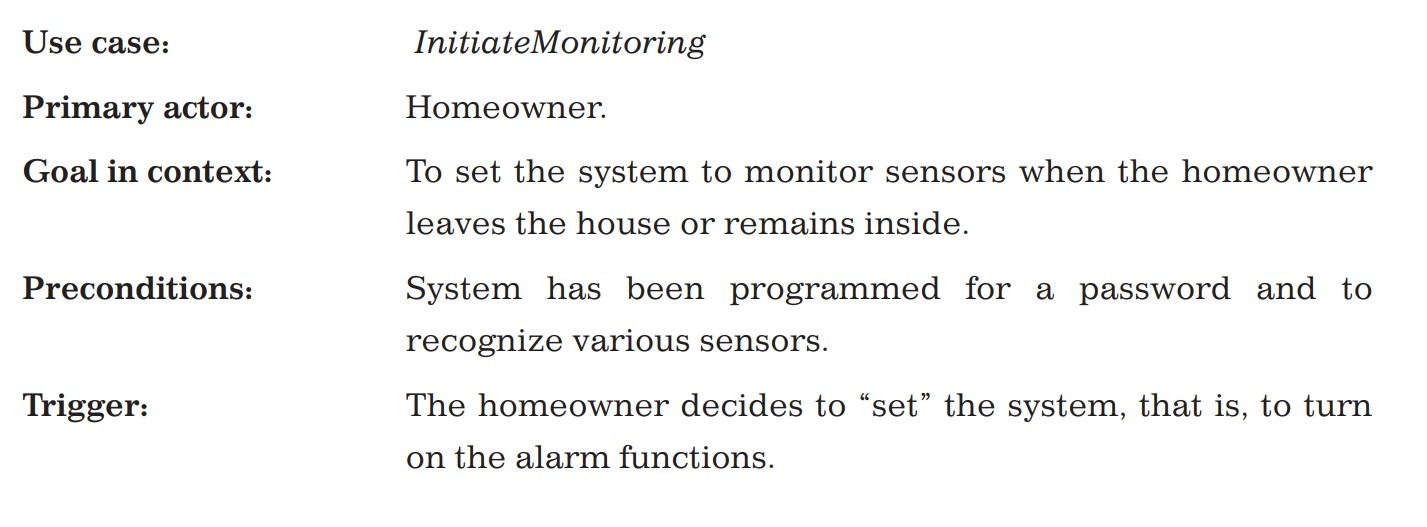
\includegraphics[scale=.4]{img/m2_17.jpg}
	%	\caption{use case diagram for SafeHome home security function }
	\end{figure}
\end{frame}
\begin{frame}{Developing use cases}
	\textbf{Scenario :}
	\begin{enumerate}
		\item Homeowner: observes control panel 
		\item Homeowner: enters password 
		\item Homeowner: selects “stay” or “away” 
		\item Homeowner: observes read alarm light to indicate that SafeHome has been armed
	\end{enumerate}
\textbf{Exceptions: }
\begin{enumerate}
	\item  Control panel is not ready: homeowner checks all sensors to determine which are 
	open; closes them. 
	\item Password is incorrect (control panel beeps once): homeowner reenters correct 
	password. 
\item Password not recognized: monitoring and response subsystem must be contacted 
	to reprogram password. 
\item Stay is selected: control panel beeps twice and a stay light is lit; perimeter sensors 
	are activated. 
	\item Away is selected: control panel beeps three times and an away light is lit; all 
	sensors are activated.
\end{enumerate}
\end{frame}
\begin{frame}{Developing use cases}
	
	\begin{figure}
		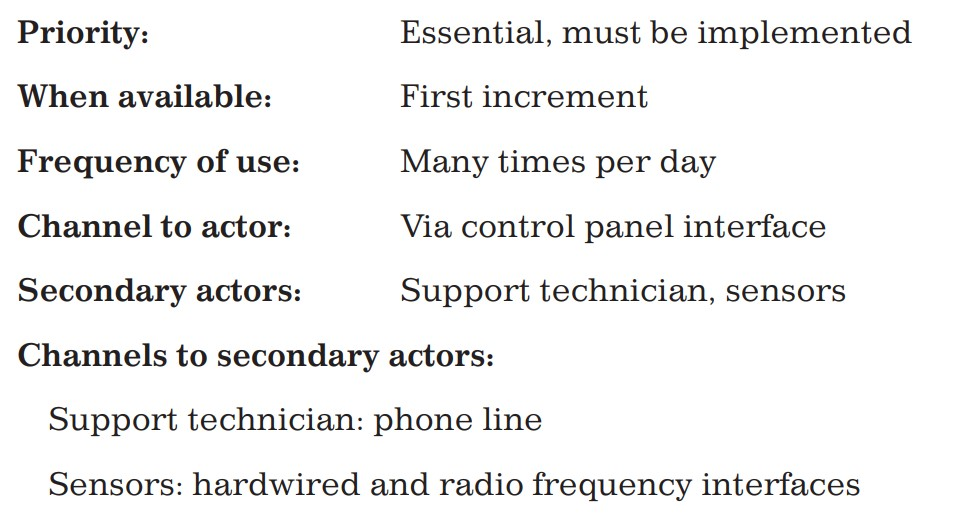
\includegraphics[scale=.5]{img/m2_18.jpg}
		%	\caption{use case diagram for SafeHome home security function }
	\end{figure}
\end{frame}
\begin{frame}{Developing use cases}
	\textbf{Open issues: }
	\begin{itemize}
		\item Should there be a way to activate the system without the use of a password or with 
		an abbreviated password? 
	\item Should the control panel display additional text messages? 
	\item How much time does the homeowner have to enter the password from the time the 
		first key is pressed? 
	\item Is there a way to deactivate the system before it actually activates? 
	\end{itemize}
\end{frame}
\begin{frame}{Software Requirements Specification Template}
\begin{figure}
	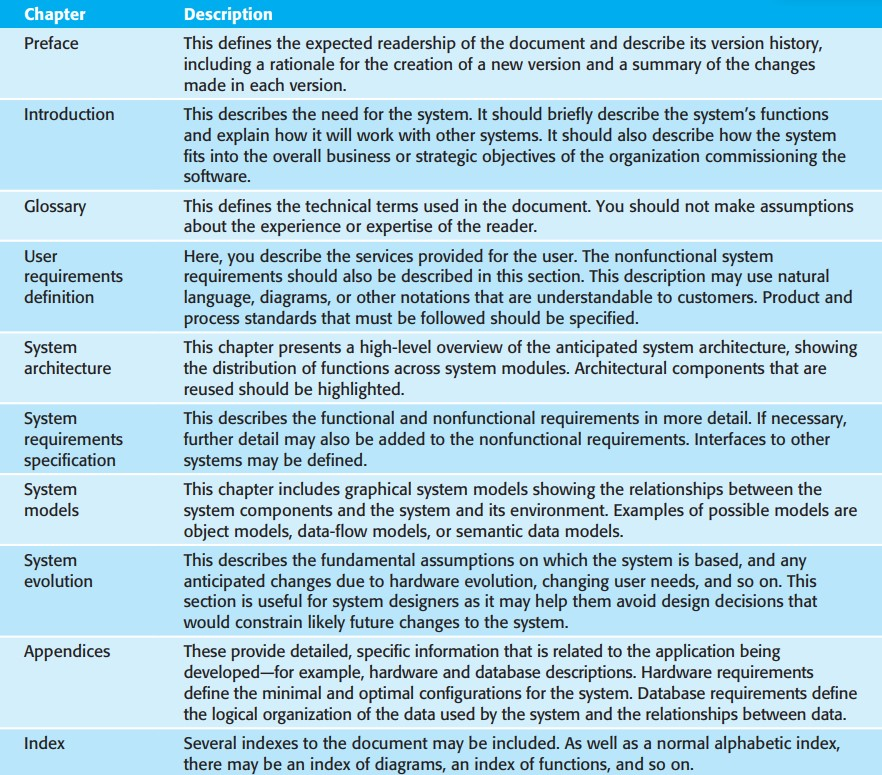
\includegraphics[scale=.42]{img/m2_32.jpg}
		\caption{The structure of a requirements document }
\end{figure}
\end{frame}


\section{Personas, Scenarios and Stories ,Feature Identification}
\begin{frame}{Personas, Scenarios and Stories ,Feature Identification}
	\textbf{personas, scenarios, and user stories lead to features 
		that might be implemented in a software product}
	\begin{figure}
		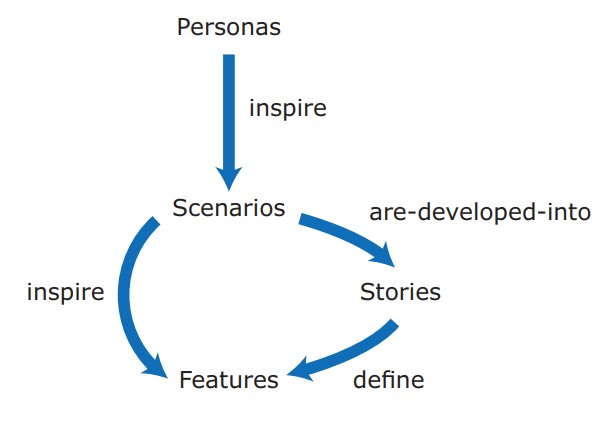
\includegraphics[scale=.5]{img/m2_19.jpg}
			\caption{From personas to features }
	\end{figure}
\end{frame}
\begin{frame}{Personas}
	\textbf{Personas}
	\begin{itemize}
		\item Personas are about “\textbf{\textit{imagined users,” character portraits of types of user that you think might adopt your product.}}
		\begin{itemize}
			\item \textbf{Example:} if your product is aimed at\textit{ managing appointments for dentists}, you might create a \textit{ dentist persona, a receptionist persona, and a patient persona}. 
		\end{itemize}
	\item Personas of different types of users help you imagine what these 
	users may want to do with your software and how they might use it.
	\item They also help you envisage difficulties that users might have in 
	understanding and using product features.
	\end{itemize}
\end{frame}
\begin{frame}{Personas}
	\textbf{Persona should include the following :}
	\begin{itemize}
		\item Description about the the users’ backgrounds
		\item Description about why the users might want to use your product
		\item Description about their education and technical skills.
	\end{itemize}

\end{frame}
\begin{frame}{Personas}
	\textbf{Persona descriptions}
	\begin{itemize}
		\item A persona should ‘\textbf{paint a picture’ of a type of product user}. 
		\item They should be relatively \textbf{short and easy-to-read}.
		\item Should describe their \textbf{background} and \textbf{why they might want to use your product}. 
		\item These help you assess whether or not a software feature is likely to be useful, understandable and usable by typical product users. 
		
	\end{itemize}
	
\end{frame}
\begin{frame}{Personas}
	\textbf{Persona descriptions}
	\begin{figure}
	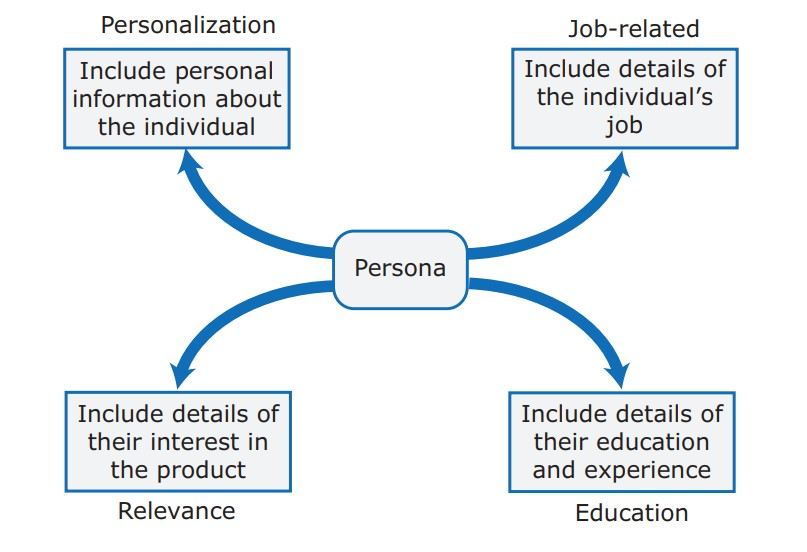
\includegraphics[scale=.5]{img/m2_21.jpg}
	\caption{Persona descriptions}
\end{figure}
	
\end{frame}
\begin{frame}{Personas}
	\textbf{Persona descriptions}
	\begin{figure}
		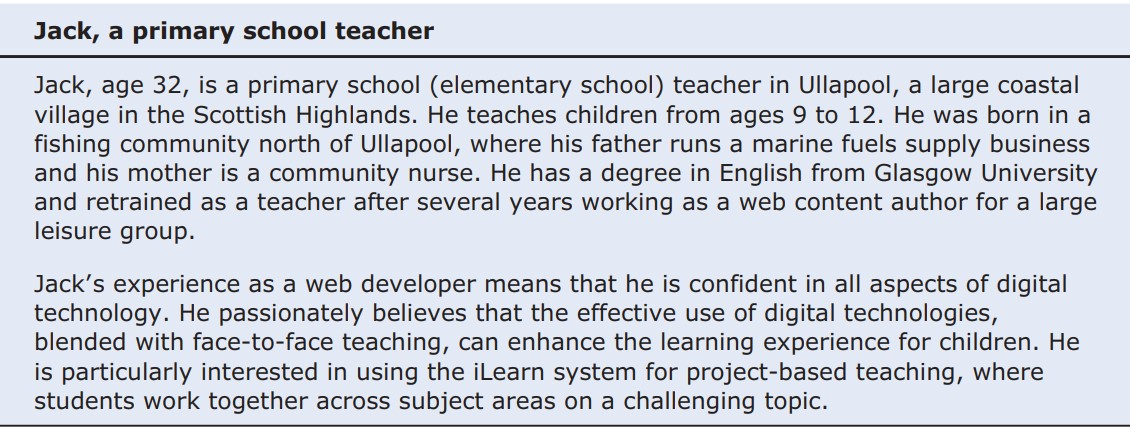
\includegraphics[scale=.5]{img/m2_20.jpg}
		\caption{Persona descriptions}
	\end{figure}
	
\end{frame}
\begin{frame}{Personas}
	\textbf{Persona descriptions}
	\begin{figure}
		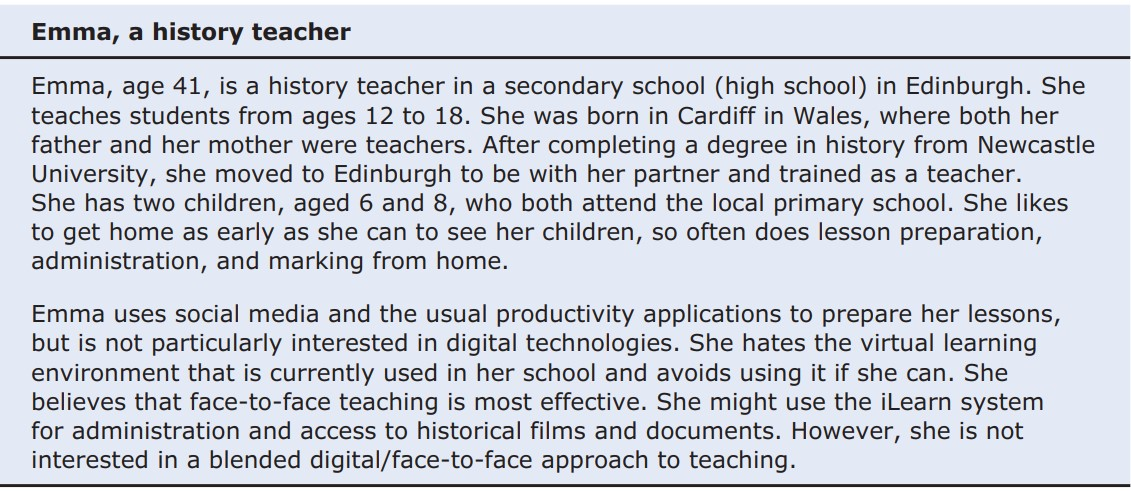
\includegraphics[scale=.5]{img/m2_22.jpg}
		\caption{A persona for a history teacher}
	\end{figure}
	
\end{frame}
\begin{frame}{Personas}
	\textbf{Persona descriptions}
	\begin{figure}
		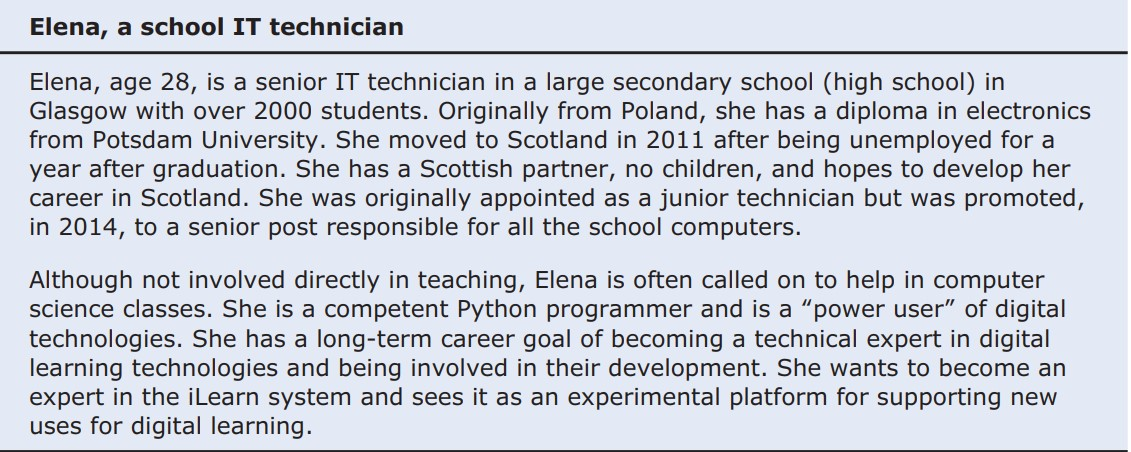
\includegraphics[scale=.5]{img/m2_23.jpg}
		\caption{A persona for an IT technician}
	\end{figure}
	
\end{frame}
\begin{frame}{Scenarios}
	\textbf{Scenarios}
	\begin{itemize}
		\item A scenario is a \textbf{narrative} that \textbf{describes how a user, or a group of users, might use your system. }
		\item There is no need to include everything in a scenario – the scenario isn’t a system specification. 
		\item It is simply a \textbf{description} of a situation \textbf{where a user is using your product’s features to do something that they want to do}.
		\item Scenario descriptions may vary in length \textbf{from two to three paragraphs up to a page of text.}
		
	\end{itemize}
	
\end{frame}
\begin{frame}{Scenarios}
	\textbf{Scenarios Cont..}
	\begin{itemize}
		\item An \textbf{imagined or projected sequence of events},
		\item Narrative, high-level scenarios, are primarily a means of facilitating 
		communication and stimulating design creativity. 
		\item They are effective in communication because they are 
		understandable and accessible to users and to people responsible for 
		funding and buying the system.
		\item Like personas, they help developers to gain a shared understanding of 
		the system that they are creating. 
		\item Scenarios are not specifications. They lack detail, they may be 
		incomplete, and they may not represent all types of user interactions.

	\end{itemize}
	
\end{frame}

\begin{frame}{Scenarios}
	%\textbf{Scenarios}
		\begin{figure}
		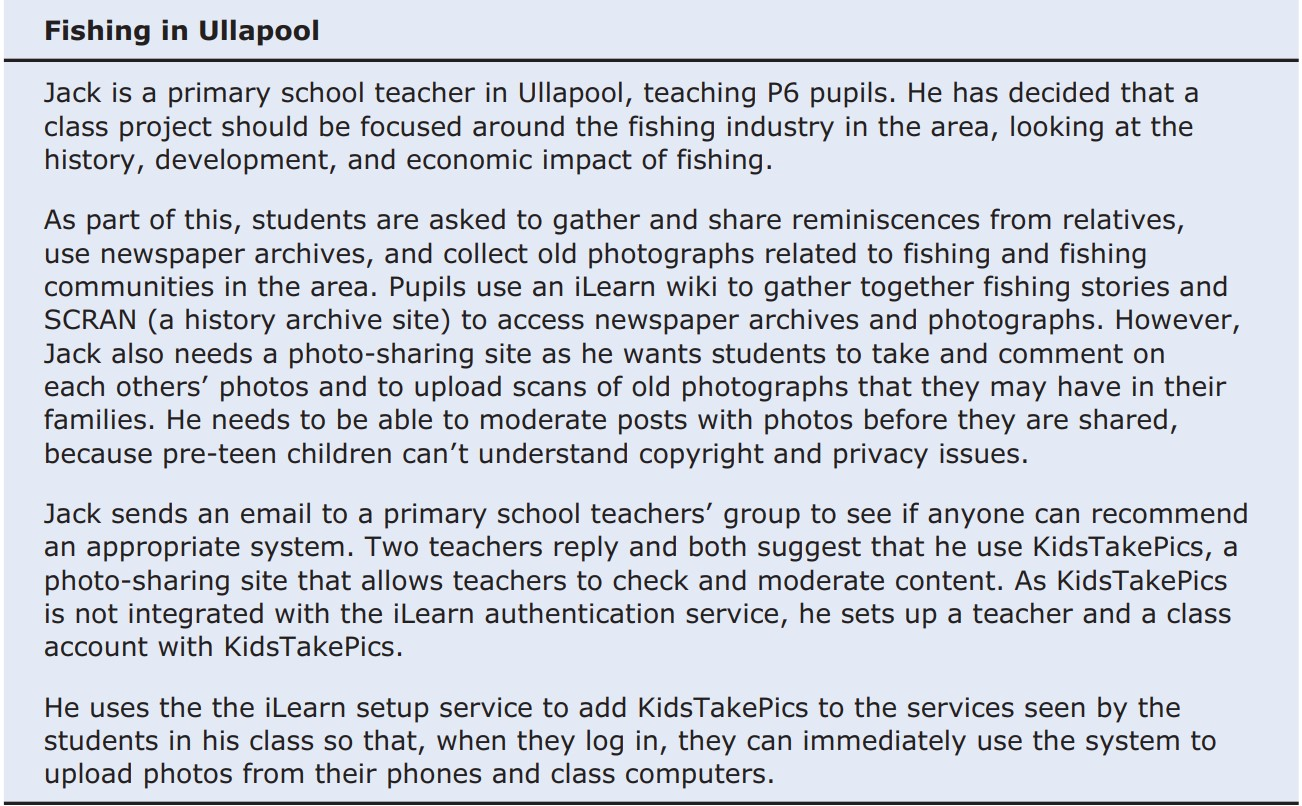
\includegraphics[scale=.4]{img/m2_25.jpg}
		\caption{Jack’s scenario: Using the iLearn system for class projects}
	\end{figure}
	
\end{frame}

\begin{frame}{Scenarios}
		\textbf{Elements of scenario}
	\begin{itemize}
		\item A brief statement of the overall objective.
		\begin{itemize}
			\item  In Jack’s scenario, this is to support a class project on the fishing industry.
		\end{itemize}
		\item References to the persona involved (Jack) so that you can get information 
		about the capabilities and motivation of that user.
		\item Information about what is involved in doing the activity.
		\begin{itemize}
			\item For example, 
			in Jack’s scenario, this involves gathering reminiscences from relatives, 
			accessing newspaper archives, and so on.
		\end{itemize} 
		\item If appropriate, an explanation of problems that can’t be readily 
		addressed using the existing system.
		\begin{itemize}
			\item  Young children don’t understand issues such as copyright and privacy, so photo sharing requires a site 
			that a teacher can moderate to make sure that published images are legal 
			and acceptable.
		\end{itemize}
		\item A description of one way that the identified problem might be addressed. 
		\begin{itemize}
			\item This may not always be included especially if technical knowledge is 
			needed to solve the problem. In Jack’s scenario, the preferred approach 
			is to use an external tool designed for school students.
		\end{itemize}
		
	\end{itemize}
	
\end{frame}
\begin{frame}{Scenarios}
	%	\textbf{Scenarios}
	\begin{figure}
		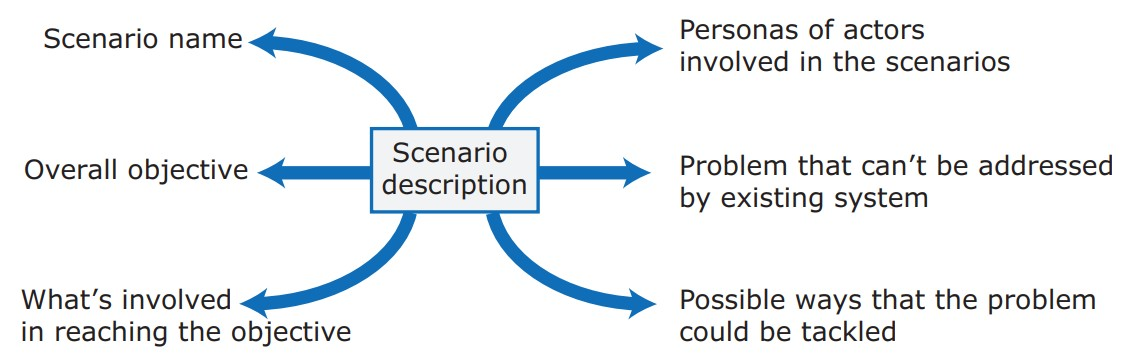
\includegraphics[scale=.5]{img/m2_24.jpg}
		\caption{Elements of a scenario description}
	\end{figure}
	
\end{frame}
\begin{frame}{Scenarios}
		\textbf{Writing scenarios}
		\begin{itemize}
			\item Scenarios should always be written from the \textbf{user’s perspective} and should 
			be based on identified personas or real users.
			\item Scenario writing is not a systematic process and different teams approach 
			it in different ways.
			\item Writing scenarios always gives you ideas for the features that you can 
			include in the system.
			\item Start with the personas that you have created.
			\item Try to imagine several scenarios for each persona.
			\item Not necessary to include every details you think users might do with your 
			product.
			
		\end{itemize}
	
	
\end{frame}
\begin{frame}{Scenarios}
	%	\textbf{Scenarios}
	\begin{figure}
		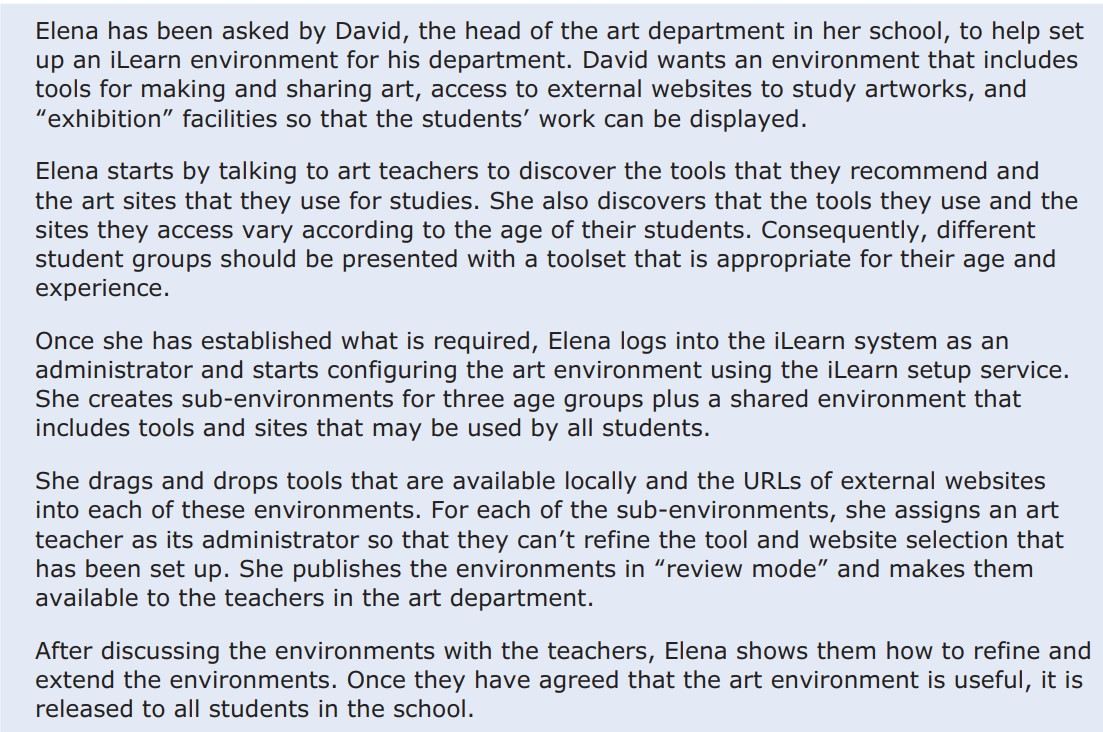
\includegraphics[scale=.45]{img/m2_26.jpg}
		\caption{Elena’s scenario: Configuring the iLearn system}
	\end{figure}
	
\end{frame}
\begin{frame}{User stories}
		\textbf{User stories}
	\begin{itemize}
		\item A user story is a well-formed, \textbf{short and simple description of a software requirement} from the \textbf{perspective of an end-user}, written in an \textbf{informal and natural language}. 
		\item User stories are not intended for planning but for helping with feature 
		identification. 
		\item Aim to develop stories that are helpful in one of 2 ways:
		\begin{itemize}
			\item as a way of extending and adding detail to a scenario; 
			\item as part of the description of the system feature that you have identified.
		\end{itemize}
	\end{itemize}
\end{frame}

\begin{frame}{User stories}
	\begin{figure}
	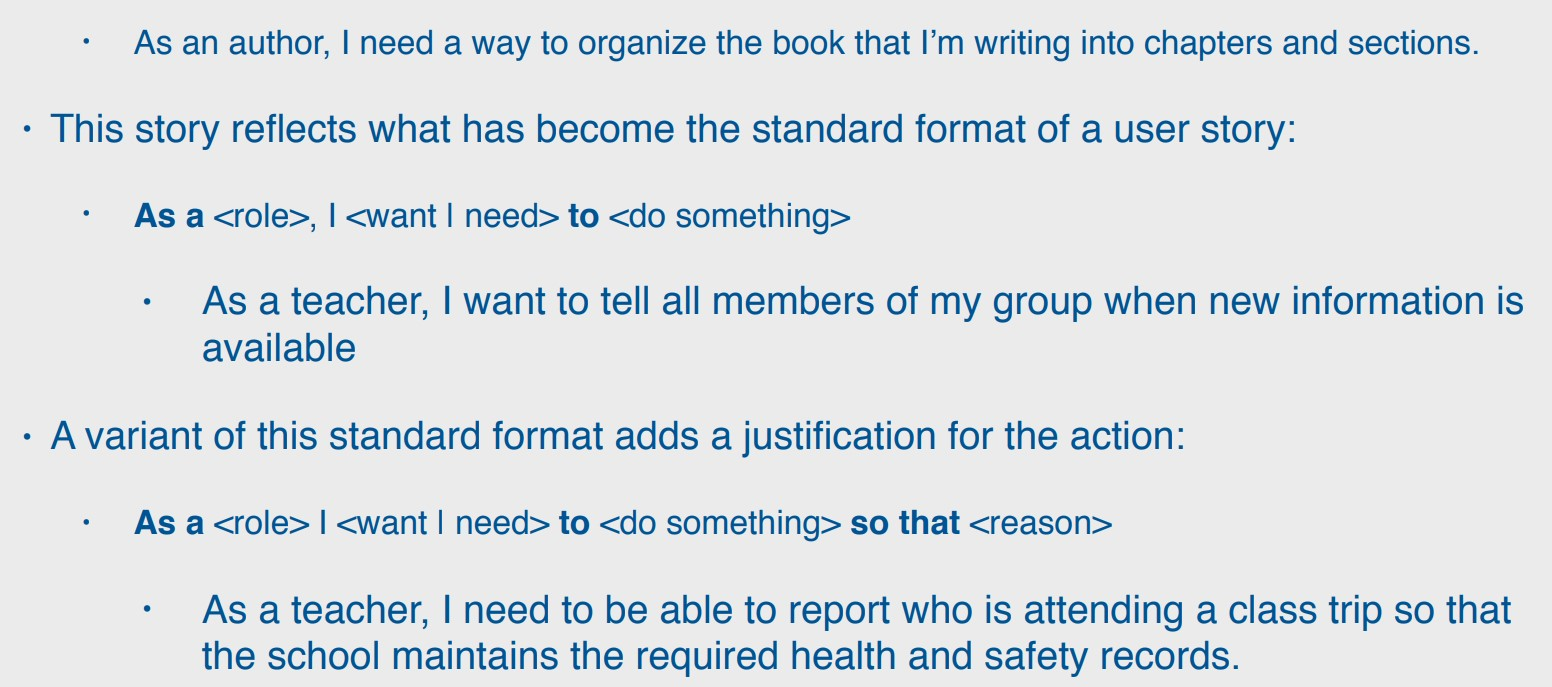
\includegraphics[scale=.35]{img/m2_43.jpg}
	%\caption{Elena’s scenario: Configuring the iLearn system}
\end{figure}
\end{frame}


\begin{frame}{User stories}
	\textbf{User stories cont..}
	\begin{itemize}
		\item When you define user stories from a scenario, you provide more 
		information to developers to help them design the product’s features.
		\item If you are writing stories to be part of a product backlog, you should 
	\textbf{	avoid negative stories.}
		\item Scenarios and stories are helpful in both choosing and designing 
		system features. 
		\item Scenarios and user stories can be thought of as “tools for thinking” 
		about a system rather than a system specification. They don’t have to 
		be complete or consistent, and there are no rules about how many of 
		each you need.
	\end{itemize}
\end{frame}
\begin{frame}{User stories}
		\begin{figure}
		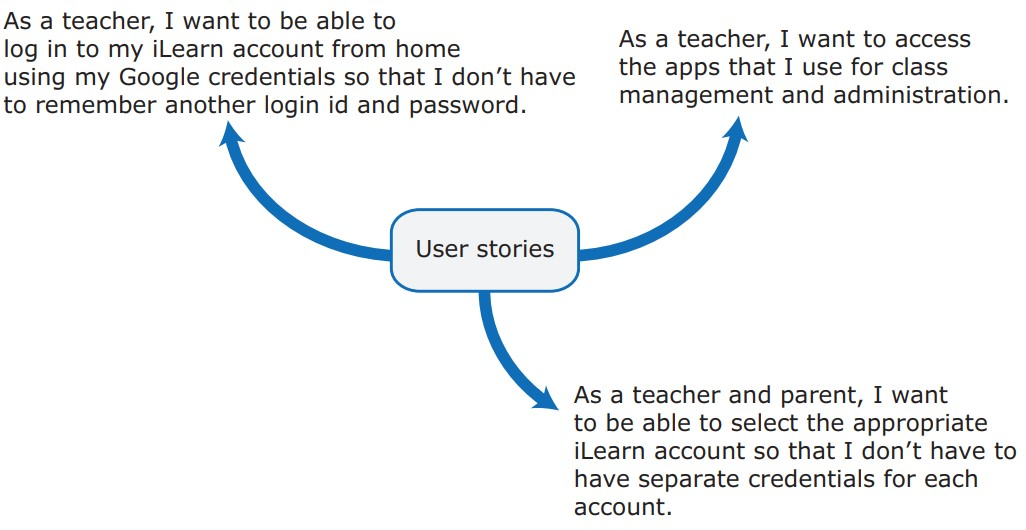
\includegraphics[scale=.45]{img/m2_27.jpg}
		\caption{User stories from Emma’s scenario}
	\end{figure}
\end{frame}
\begin{frame}{User stories}
\textbf{User stories in planning}
\begin{itemize}
	\item An important use of user stories is in planning.
	\begin{itemize}
		\item Many users of the Scrum method represent the product backlog as a set of user stories. 
	\end{itemize}
\item User stories should focus on a clearly defined system feature or aspect of a feature that can be implemented within a single sprint. 
\item If the story is about a more complex feature that might take several sprints to implement, then it is called an epic.

\end{itemize}
\end{frame}

\begin{frame}{Feature identification}
	A “feature” can be defined as: “A discrete piece of functionality desired by stakeholders”\\
	\textbf{Feature identification}
	\begin{itemize}
		\item A feature is a way of allowing users to access and use your product’s 
		functionality so that the feature list defines the overall functionality of the 
		system.
		\item Identify the product features that are independent, coherent and relevant:
		\begin{itemize}
			\item \textbf{Independence:} A feature should not depend on how other system features are 
				implemented and should not be affected by the order of activation of other 
				features.
			\item \textbf{Coherence Features:}Features  should be linked to a single item of functionality. They 
				should not do more than one thing, and they should never have side effects.

			\item \textbf{Relevance System features:}Features  should reflect the way users normally carry out 
				some task. They should not offer obscure functionality that is rarely required.
		\end{itemize}
	\end{itemize}
\end{frame}

\begin{frame}{Feature identification}
	\begin{figure}
		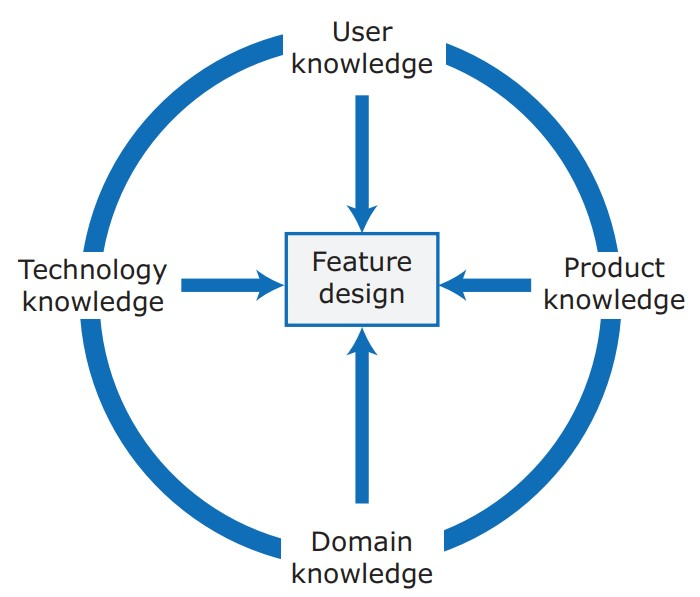
\includegraphics[scale=.45]{img/m2_28.jpg}
		\caption{Feature design}
	\end{figure}
\end{frame}
\begin{frame}{Feature identification}
	\begin{figure}
		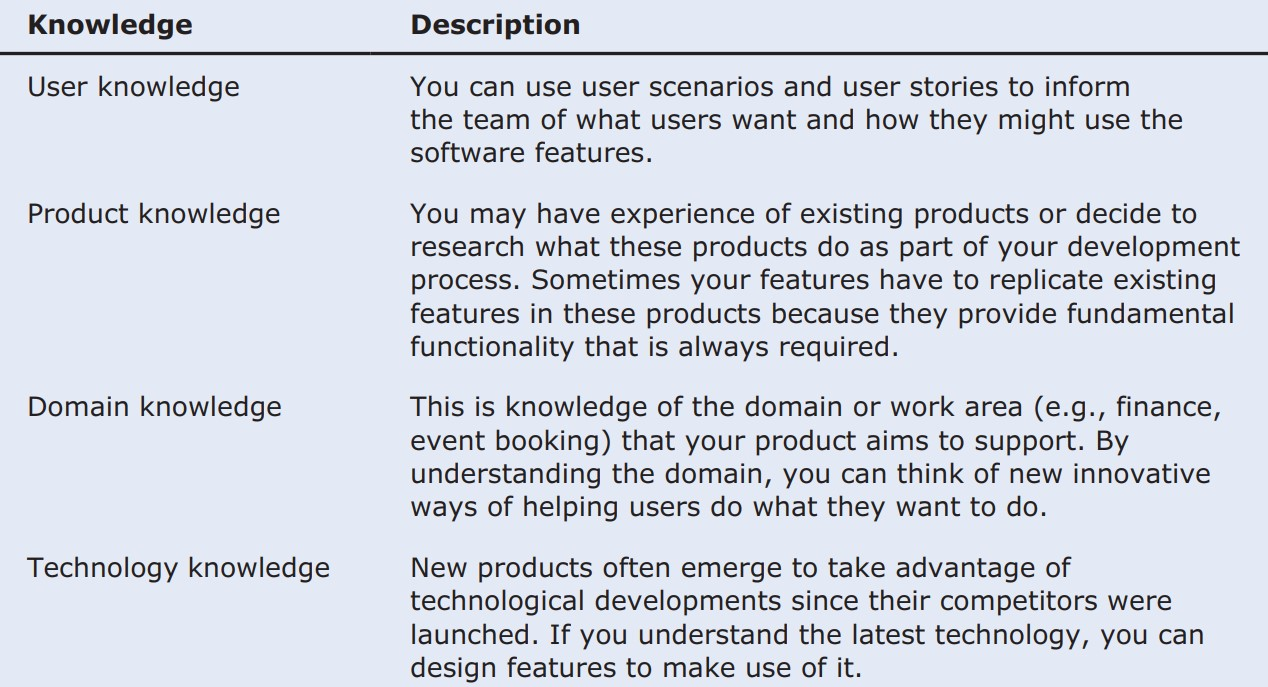
\includegraphics[scale=.45]{img/m2_29.jpg}
		\caption{Knowledge required for feature design}
	\end{figure}
\end{frame}
\begin{frame}{Feature identification}
	\textbf{Factors in feature set design}
	\begin{figure}
		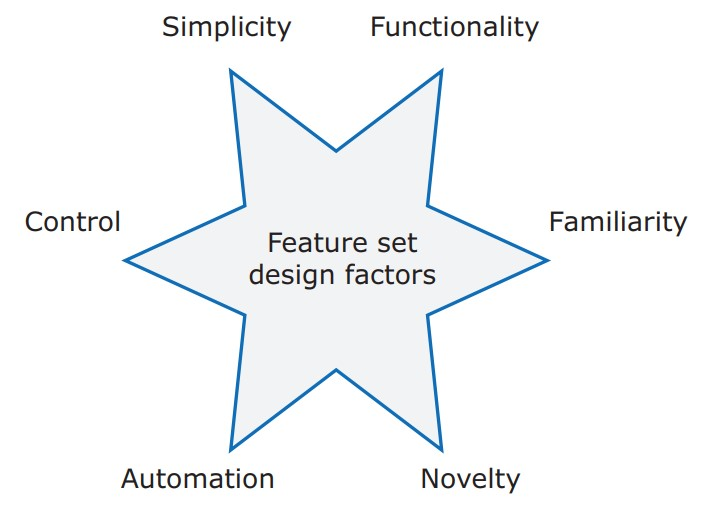
\includegraphics[scale=.45]{img/m2_30.jpg}
		\caption{Factors in feature set design}
	\end{figure}
\end{frame}
\begin{frame}{Feature identification}
	\textbf{Factors in feature set design}
	\begin{itemize}
		\item \textbf{Simplicity and functionality }
		\begin{itemize}
			\item Find a balance between providing a \textbf{simple, easy-to-use} system and \textbf{including enough functionality to attract users} with a variety of needs.
		\end{itemize}
		\item \textbf{Familiarity and novelty}
		\begin{itemize}
			\item Users prefer that new software should support the \textbf{familiar everyday tasks that are part of their work or life}. Find a \textbf{balance between familiar features and new features} that convince users that your product can do more than its competitors. 
		\end{itemize}
		\item \textbf{Automation and control}
		\begin{itemize}
			\item Some users like automation, where the software does things for them. Others prefer to have control. 
		\end{itemize}
	\end{itemize}
\end{frame}
\begin{frame}{Feature identification}
	\textbf{Feature creep}
	\begin{itemize}
		\item Feature creep, more commonly known as scope creep, refers to when you \textbf{add excessive features to a product} that make it too \textbf{complicated or difficult} to use. 
		\item Too many features make products hard to use and understand
		\item There are 3 reasons why feature creep occurs:
		\begin{itemize}
			\item Product managers are \textbf{reluctant to say ‘no’} when users ask for specific features.
			\item Developers\textbf{ try to match features in competing products}.
			\item The product includes \textbf{features to support} both \textbf{inexperienced and experienced users}.
			
		\end{itemize}
	\end{itemize}
\end{frame}
\begin{frame}{Feature identification}
%	\textbf{Factors in feature set design}
	\begin{figure}
		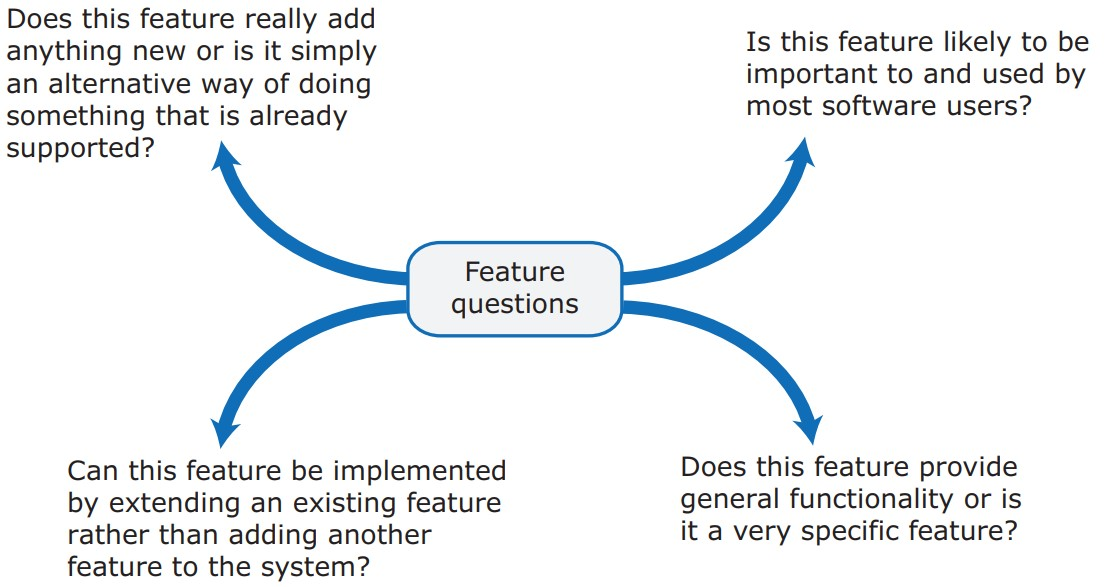
\includegraphics[scale=.45]{img/m2_31.jpg}
		\caption{Avoiding feature creep}
	\end{figure}
\end{frame}
\begin{frame}{Feature identification}
		\textbf{The feature list}
		\begin{itemize}
			\item The output of the feature identification process should be a list of features that you use for designing and implementing your product. 
			\item There is no need to go into a lot of detail about the features at this stage. You add detail when you are implementing the feature. 
			\item You can describe features using a standard input-action-output template by using structured narrative descriptions or by a set of user stories.
		\end{itemize}
\end{frame}
\begin{frame}{Feature identification}
	\textbf{Feature derivation}
	\begin{itemize}
		\item Features can be identified \textbf{directly from the product vision or from scenarios}.
		\item You can\textbf{ highlight phrases in narrative description} to identify features to be included in the software.
		\begin{itemize}
			\item You should think about the features needed to support user actions, identified by active verbs, such as use and choose.
		\end{itemize}
	\end{itemize}
\end{frame}
\section{Design concepts}
\begin{frame}{Design concepts}
	\textbf{Design concepts}
	\begin{itemize}
		\item Design with context of software engineering
		\item The Design process
		\item Design Concepts
		\item The Design Model
	\end{itemize}
\end{frame}
\begin{frame}{Design concepts}
	\textbf{Design}
	\begin{itemize}
		\item Software design is a process to\textbf{ transform user requirements into some suitable form}, which\textbf{ helps the programmer in software coding and implementation}.
		\item The design    model \textbf{provides} detail about \textbf{software architecture, data structures, 
			interfaces, and components} that are \textbf{necessary to implement the 
			system.}
		\item \textbf{The goal of design}\\To produce a model or representation that exhibits
		\begin{itemize}
			\item \textbf{Firmness:} A program should not have any bugs that inhibit its function. 
			\item \textbf{Commodity:} A useful or valuable thing
			\item \textbf{Delight:} The experience of using the program should be a pleasurable one.
		\end{itemize}
	\end{itemize}
\end{frame}
\begin{frame}{Design concepts}
	\textbf{Design Within the Context of Software Engineering}
	\begin{itemize}
		\item Software design is the last software engineering action within the modeling activity       and sets the stage for construction (code generation and testing).
	\end{itemize}
\end{frame}
\begin{frame}{Design Within the Context of Software Engineering}
	\begin{figure}
	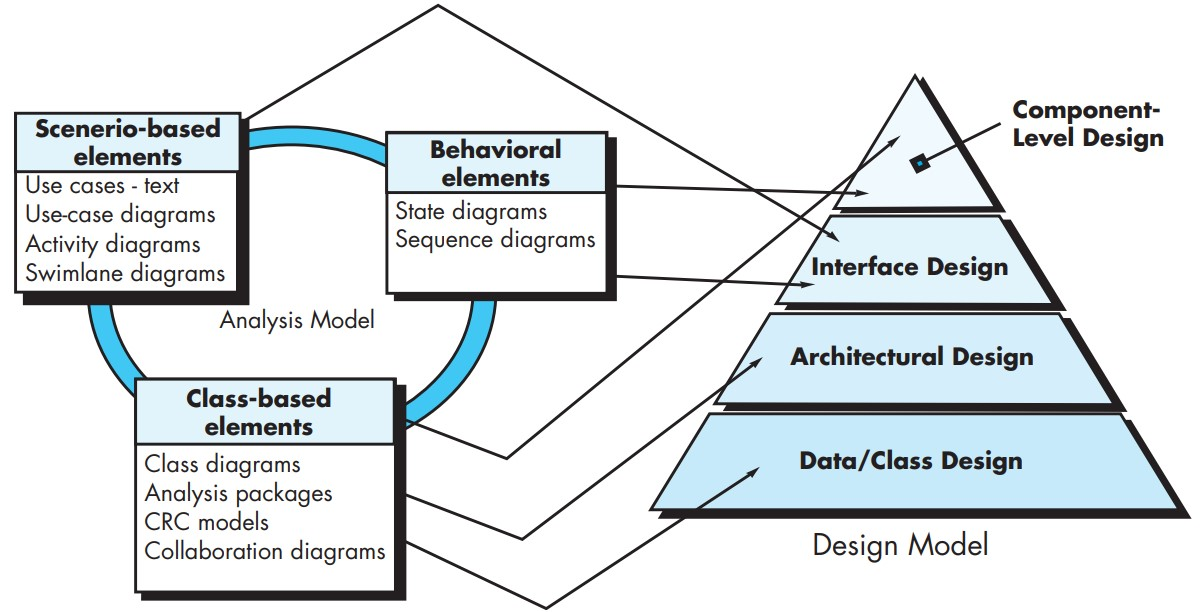
\includegraphics[scale=.45]{img/m2_33.jpg}
	\caption{Translating the requirements model into the design model }
\end{figure}
\end{frame}
\begin{frame}{Design Within the Context of Software Engineering}
	The requiremets model haning the following basic elements,which feed the design task.
	\begin{itemize}
		\item Scenario-based
		\item Class-based and
		\item behavioral elements,
	\end{itemize}
The design process will produces 4 different design model
\begin{itemize}
	\item \textbf{Data/Class design} – transforms analysis classes into implementation classes and data structures
	\item \textbf{Architectural design} – defines relationships among the major software structural elements
	\item \textbf{Interface design} – defines how software elements, hardware elements, and end-users communicate
	\item  \textbf{Component-level design} – transforms structural elements into procedural descriptions of software components
\end{itemize}
\end{frame}
\begin{frame}{Design concepts}
	\textbf{THE DESIGN PROCESS}
	\begin{itemize}
		\item Software design is an iterative process through which requirements are translated into a “blueprint” for constructing the software. 
	\end{itemize}
\textbf{Software Quality Guidelines and Attributes }
\begin{itemize}
	\item Three characteristics used for evaluation of quality
	\begin{enumerate}
		\item The design should \textbf{implement all of the explicit requirements contained in the 
			requirements model}, and it must accommodate all of the implicit requirements desired by 
		stakeholders.
		\item The design should be \textbf{readable and understandable} for those who generate code and test 
		the software.
		\item The design \textbf{should provide a complete picture of the software}, addressing the data, 
		functional, and behavioral domains from an implementation perspective.
	\end{enumerate}
\end{itemize}
\end{frame}
\begin{frame}{THE DESIGN PROCESS}
	\textbf{Quality Guidelines:}
	\begin{itemize}
		\item[1] A design is generated using the recognizable architectural styles and compose a good design characteristic of components and it is implemented in evolutionary manner for testing.
	
		\item[2] A design should be modular; i.e., the software should be logically partitioned into elements or 
		subsystems.
		\item[3] A design should contain distinct representations of data, architecture, interfaces, and 
		components.
	
	\end{itemize}
\end{frame}
\begin{frame}{THE DESIGN PROCESS}
	\textbf{Quality Guidelines cont..}
	\begin{itemize}
		\item[4] A design should lead to data structures that are appropriate for the classes to be implemented 
		and are drawn from recognizable data patterns. 
		\item[5] A design should lead to components that exhibit independent functional characteristics.
		\item[6] A design should lead to interfaces that reduce the complexity of connections between 
		components and with the external environment.
		\item[7] A design should be derived using a repeatable method that is driven by information obtained 
		during software requirements analysis.
		\item[8] A design should be represented using a notation that effectively communicates its meaning.
	\end{itemize}
\end{frame}
\begin{frame}{THE DESIGN PROCESS}
	\textbf{Quality Attributes:}
	\begin{enumerate}
		\item \textbf{Functionality:}  assessed by evaluating the feature set and capabilities of  the program, the generality of the functions that are delivered, and the  security of the overall system.
		\item \textbf{Usability:} assessed by considering human factors , overall aesthetics,
		consistency, and documentation.
		\item \textbf{Reliability:} evaluated by measuring the frequency and severity of failure,  the accuracy of output results, the mean-time-to-failure (MTTF), the ability  to recover from failure, and the predictability of the program.
		\item \textbf{Performance:} measured using processing speed, response time, resource  consumption, throughput, and efficiency.
		\item \textbf{Supportability:} combines extensibility, adaptability, and serviceability.
		
	\end{enumerate}
\end{frame}
\begin{frame}{Design concepts}
	\textbf{Design concepts}\\An overview of fundamental software design concepts:
\begin{enumerate}
	\item Abstraction
	\item Architecture
	\item Patterns
\item Separation of Concerns
\item Modularity
	\item Information Hiding
	\item Functional Independence
\item Refinement
\item Aspects
\item Refactoring
\item Object-Oriented Design Concepts
\item Design Classes
\item Dependency Inversion
\item Design for Test
\end{enumerate}

\end{frame}
\begin{frame}{Design concepts}
	\textbf{Abstraction}
	\begin{itemize}
		\item Many levels of abstraction can be posed
		\begin{itemize}
			\item At the highest level of abstraction, a solution is stated in broad terms using 
			the language of the problem environment. 
			\item At lower levels of abstraction, a more detailed description of the solution is 
			provided.
		\end{itemize}
	\item Create both procedural and data abstractions.
	\begin{itemize}
		\item \textbf{Procedural abstraction:} a sequence of instructions that have a specific 
		and limited function.
		\item \textbf{Data abstraction:} a named collection of data that describes a data 
			object. 
	\end{itemize}
	\end{itemize}
\end{frame}
\begin{frame}{Design concepts}
	\textbf{Architecture}
	\begin{itemize}
		\item The complete structure of the software is known as software architecture.
		\item It consists of components,connectiors, and the relationship between them
	
		\item Shaw and Garlan describe a set of properties that should be specified as part of an architectural 
		design. 
		\begin{itemize}
			\item \textbf{Structural properties define} “the components of a system (e.g., modules, objects, filters) 
			and the manner in which those components are packaged and interact with one another.”.
			\item \textbf{Extra-functional properties address} “how the design architecture achieves requirements 
			for performance, capacity, reliability, security, adaptability, and other system 
			characteristics. 
			\item \textbf{Families of related systems} “draw upon repeatable patterns that are commonly encountered 
			in the design of families of similar systems.”
		\end{itemize}
	\end{itemize}
\end{frame}
\begin{frame}{Design concepts}
	\textbf{Architecture Cont..}
	\begin{itemize}
		\item The architectural design can be represented using one 
		or more of a number of different models.
		\begin{itemize}
			\item \textbf{Structural models:} represent architecture as an organized collection 
			of program components. 
			\item \textbf{Framework models:} increase the level of design abstraction by 
			attempting to identify repeatable architectural design frameworks 
			(patterns) that are encountered in similar types of applications.
			\item \textbf{Dynamic models:} address the behavioral aspects of the program 
			architecture, indicating how the structure or system configuration may 
			change as a function of external events. 
			\item \textbf{Process models} focus on the design of the business or technical 
			process that the system must accommodate. 
			\item \textbf{Functional models:} used to represent the functional hierarchy of a 
			system.
			
		\end{itemize}
	\end{itemize}
\end{frame}
\begin{frame}{Design concepts}
	\textbf{Patterns:}
	\begin{itemize}
		\item A design structure that solves a perticular design problem within a specific context
		\item It provides a description that enables a designer to determine whether the pattern is applicable,
		\item whether the pattern can be reused, and 
		\item whether the pattern can serve as a guide for developing for similar pattern
	\end{itemize}
\end{frame}
\begin{frame}{Design concepts}
	\textbf{Separation of Concerns:}
	\begin{itemize}
		\item Separation of concerns is a design concept that suggests that any complex 
		problem can be more easily handled if it is subdivided into pieces that can each be 
		solved and/or optimized independently. 
		\item A concern is a feature or behavior that is 
		specified as part of the requirements model for the software.
		\item  By separating concerns into smaller, and therefore more manageable pieces, a problem 
		takes less effort and time to solve.
	\end{itemize}
\end{frame}

\begin{frame}{Design concepts}
	\textbf{Modularity:}
	\begin{itemize}
		\item Software is divided into separately named and addressable components, sometimes called 
		modules, that are integrated to satisfy problem requirements. 
		\item Modularity is the single attribute of software that allows a program to be 
		intellectually manageable
		
	\end{itemize}
	\begin{figure}
	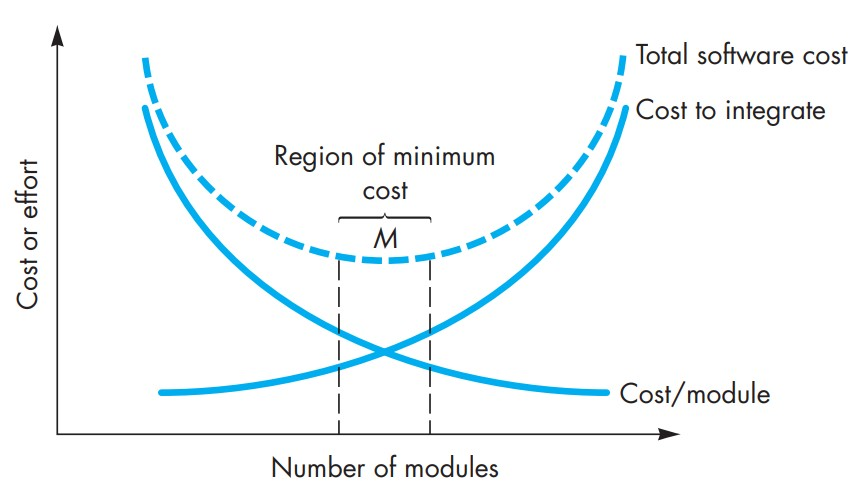
\includegraphics[scale=.45]{img/m2_34.jpg}
	\caption{Modularity 
		and software 
		cost  }
\end{figure}
\end{frame}
\begin{frame}{Design concepts}
	\textbf{Information Hiding :}
	\begin{itemize}
		\item The designing of modules so that information (algorithms and data)  contained within a module is inaccessible to other modules that have no  need for such information.
		\item This enforces access constraints to both procedural(ie. implementation)details and local data structure
	\end{itemize}

\end{frame}
\begin{frame}{Design concepts}
	\textbf{Functional Independence :}
	\begin{itemize}
		\item The functional independence is the concept of separation and related to the concept of modularity, abstraction and information hiding.
		\item Independence is assessed using 2 qualitative criteria:
		\begin{itemize}
			\item \textbf{Cohesion:}  an indication of the relative functional strength of a module.
			\begin{itemize}
				\item A cohesive module performs a single task and it requires a small interaction with the other components in other parts of the program.
			\end{itemize}
			\item \textbf{Coupling:} an indication of the relative interdependence among modules.
			\begin{itemize}
				\item Coupling is an indication of interconnection between modules in a structure of software.
			\end{itemize}
		\end{itemize}
	\end{itemize}
\end{frame}
\begin{frame}{Design concepts}
	\textbf{Refinement :}
	\begin{itemize}
		\item Stepwise refinement is a top-down design strategy.
		\item It is actually a process of elaboration.
		\item You begin with a statement of function (or description of information) that
		is defined at a high level of abstraction.
		\item You then elaborate on the original statement, providing more and more  detail as each successive refinement (elaboration) occurs.
		\item Abstraction and refinement are complementary concepts. 
		
		\end{itemize}
\end{frame}
\begin{frame}{Design concepts}
	\textbf{Aspects :}
	\begin{itemize}
		\item An aspect is a representation of a crosscutting concern. 
		\item A crosscutting concern is 
		some characteristic of the system that applies across many different requirements
		\item Consider 2 requirements, A and B. Requirement A crosscuts requirement B  “if a software decomposition [refinement] has been chosen in which B  cannot be satisfied without taking A into account”.
		
	\end{itemize}
\end{frame}
\begin{frame}{Design concepts}
	\textbf{Refactoring :}
	\begin{itemize}
		\item A reorganization technique that simplifies the design (or code) of a  component without changing its function or behavior.
		\item Removes redundancy, unused design elements, inefficient or unnecessary algorithms,poorly constructed or inappropriate data structures, or any other design failures
	\end{itemize}
\end{frame}
\begin{frame}{Design concepts}
	\textbf{Object-Oriented Design Concepts :}
	\begin{itemize}
		\item The object-oriented (OO) paradigm is widely used in modern software 
		engineering. 
		\item OO design concepts such as classes and objects, inheritance, 
		messages, and polymorphism, among others
	\end{itemize}
\end{frame}
\begin{frame}{Design concepts}
	\textbf{Design Classes:}
	\begin{itemize}
		\item A design class is a description of a set of objects that share the same responsibilities, relationships, operations, attributes, and semantics.
		\item 5 different types of design classes:
		\begin{itemize}
			\item  \textbf{User interface classes :} define all abstractions that are necessary for human-
			computer interaction (HCI) and often implement the HCI in the context of a metaphor.
		\item \textbf{Business domain classes :}The class identifies the attributes that are required to implement some elements of the business domain.
			\item \textbf{Process classes:} implement lower-level business abstractions required to fully
			manage the business domain classes.
			\item \textbf{Persistent classes:} represent data stores (e.g., a database) that will persist beyond  the execution of the software.
		\item \textbf{	System classes:} implement software management and control functions that enable  the system to operate and communicate within its computing environment and with  the outside world.
			
		\end{itemize}
	\end{itemize}
\end{frame}
\begin{frame}{Design concepts}
\textbf{Design Classes cont..:}
\begin{itemize}
	\item 4 characteristics of a well-formed design class:
	\begin{itemize}
		\item  Complete and sufficient
		\item Primitiveness
		\item High cohesion \textbf{(keeping parts of a code base that are related to each other in a single place.)}
		\item Low coupling \textbf{(separating unrelated parts of the code base as much as possible.)}
		
	\end{itemize}
\end{itemize}
\end{frame}
\begin{frame}{Design concepts}
	\textbf{Dependency Inversion:}
	\begin{itemize}
		\item The dependency inversion principle states:
		\begin{itemize}
			\item  High-level modules (classes)  should not depend [directly] upon low-level modules. 
			 Both should depend  on abstractions. 
			\item Abstractions should not depend on details. 
		 Details should  depend on abstractions.
		\end{itemize}
		\end{itemize}
	\textbf{Design for Test:}
	\begin{itemize}
		\item whether software design or test case design should come first.
		\item Advocates of test-driven development (TDD) write tests before implementing any 
		other code.
		\item “Test fast, fail fast, adjust fast.”
	\end{itemize}
\end{frame}
\begin{frame}{THE DESIGN MODEL}
\textbf{THE DESIGN MODEL}
\begin{itemize}
	\item The design model can be viewed in two different dimensions.
	\begin{enumerate}
		\item \textbf{Process dimension} indicates the evolution of the design model as  design tasks are executed as part of the software process.
		\item \textbf{Abstraction dimension} represents the level of detail as each element  of the analysis model is transformed into a design equivalent and then  refi ned iteratively.
		
	\end{enumerate}
\end{itemize}
\end{frame}
\begin{frame}{THE DESIGN MODEL}
		\begin{figure}
		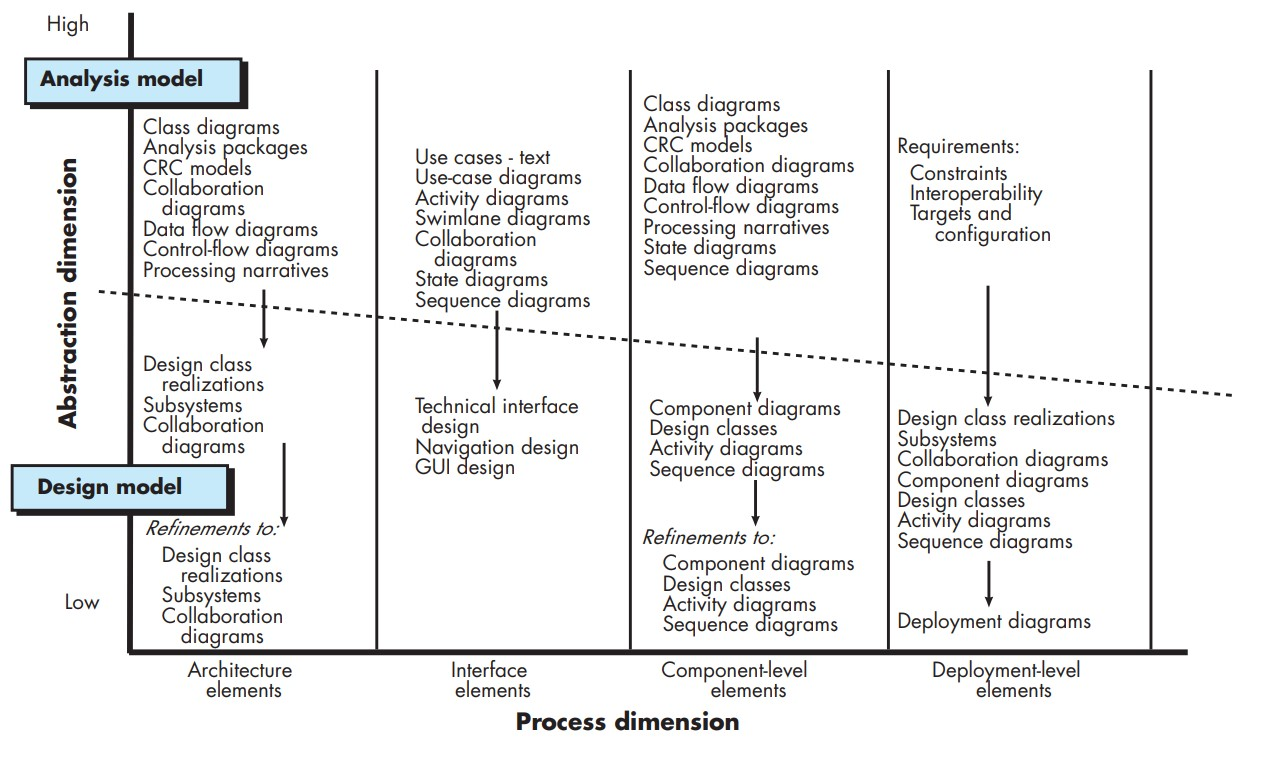
\includegraphics[scale=.4]{img/m2_35.jpg}
		\caption{Dimensions of the design model }
	\end{figure}
\end{frame}
\begin{frame}{THE DESIGN MODEL}
	\textbf{The design model has 4 major elements:}
\begin{itemize}
	\item 	Data Design Elements,
	\item Architectural Design Elements,
	\item Interface Design Elements, and
	\item Component-Level Design Elements.
\end{itemize}
\end{frame}
\begin{frame}{THE DESIGN MODEL}
	\textbf{The design model has following layered elements:}
	\begin{itemize}
		\item 	Data Design Elements,
		\begin{itemize}
			\item Creates a model of data and objects that is represented at a high level of abstraction
		\end{itemize}
		\item Architectural Design Elements,
		\begin{itemize}
			\item Depicts the overall layout of the software
		\end{itemize}
		\item Interface Design Elements, 
		\begin{itemize}
			\item Tells how information flows into and out of the system and how it is communicated among the components defined as part of the architecture
			\item includes the user interface, external interfaces, and internal interfaces
		\end{itemize}
		\item Component-Level Design Elements.
		\begin{itemize}
			\item Describes the internal details of each software component by way of data structure definitions,algorithms, and interface specifications.
		\end{itemize}
	\item Development-Level Design Elements:
	\begin{itemize}
		\item Deployment-level design elements indicate how software functionality and  subsystems will be allocated within the physical computing environment  that will support the software.
		
	\end{itemize}
	\end{itemize}
\end{frame}
\section{ARCHITECTURAL DESIGN}
\begin{frame}{ARCHITECTURAL DESIGN}
	\textbf{ARCHITECTURAL DESIGN}
	\begin{itemize}
		\item Software Architecture, 
		\item Architectural Styles, 
		\item Architectural considerations, 
		\item Architectural Design
	\end{itemize}
\end{frame}
\begin{frame}{ARCHITECTURAL DESIGN}
	\textbf{Software Architecture, }
	\begin{itemize}
		\item What is Architecture
		\item Why Is  Architecture Important?
		\item  Architectural Descriptions
		\item  Architectural Decisions
	\end{itemize}
\end{frame}
\begin{frame}{Software Architecture}
	\textbf{ What is Architecture}
	\begin{itemize}
		\item The software architecture of a program or computing system is the \textbf{structure or structures of the 
			system}, which comprise \textbf{software components}, the \textbf{externally visible properties} of those 
		components, and the \textbf{relationships among them}
		\item The architecture is not the operational software. Rather, it is a representation that enables 
		you to
		\begin{itemize}
			\item analyze the effectiveness of the design in meeting its stated requirements,
			\item consider architectural alternatives at a stage when making design 
			changes isstill relatively easy, and
			\item reduce the risks associated with the construction of the software.

		\end{itemize}
	\end{itemize}
\end{frame}
\begin{frame}{Software Architecture}
	\textbf{Why Is  Architecture Important?}
	\begin{itemize}
		\item Three Key Reasons
		\begin{itemize}
			\item  The representation of software architecture \textbf{allows the communication between all stakeholder and the developer.}
			\item The architecture \textbf{helps with early-stage decision-making} that impact on all software engineering work and it is the ultimate success of the system.
			\item  This model helps for \textbf{making further changes and adjustments}
		\end{itemize}
	\end{itemize}
\end{frame}
\begin{frame}{Software Architecture}
	\textbf{Architectural Descriptions}
	\begin{itemize}
		\item \textbf{Different stakeholders} will see an architecture from 
	\textbf{different viewpoints} that are driven by different sets of concerns.
	\item An architectural description is actually\textbf{ a set of work products} that \textbf{reflect different views of the system}.
	\end{itemize}
\end{frame}
\begin{frame}{Software Architecture}
	\textbf{Architectural Decisions:}
	\begin{itemize}
		\item Each view developed as part of an architectural description 
		\textbf{addresses a specific stakeholder concern}. 
		\item \textbf{To develop each view} the system architect \textbf{considers 
			a variety of alternatives} and \textbf{ultimately decides} on the specific \textbf{architectural features that best meet the concern}.
	\end{itemize}
\end{frame}

\begin{frame}{ARCHITECTURAL STYLES}
	\textbf{ARCHITECTURAL STYLES}
	\begin{itemize}
	%	\item The architectural style is a transformation and it is applied to the design of an entire system.
		\item The main \textbf{aim} of architectural style is \textbf{to build a structure for all components of the system}.
		\item The software that is built for computer-based systems can exhibit one of the different architectural styles. 
		\item The design categories of \textbf{architectural styles includes}:
		\begin{enumerate}
			\item a \textbf{set of components}
			\item a \textbf{set of connectors} that enables" communication and coordination
			\item \textbf{constraints} that define \textbf{how components} can be \textbf{integrated} to form the system
			\item \textbf{Semantic models} to understand the overall properties of a system
		\end{enumerate}
	\end{itemize}
\end{frame}
\begin{frame}{ARCHITECTURAL STYLES}
%	\textbf{ARCHITECTURAL STYLES}
	\begin{itemize}
		\item Taxonomy of architectural styles
		\begin{itemize}
			\item Data-centered architectures. 
			\item Data-flow architectures.
			\item Call and return architectures.
			\item Object-oriented architectures.
			\item Layered architectures
		\end{itemize}
	\end{itemize}
\end{frame}
\begin{frame}{ARCHITECTURAL STYLES}
	\textbf{Data-centered architectures. }
	\begin{itemize}
		\item \textbf{A data store} (e.g., a file or database) resides \textbf{at the 
			center} of this architecture and is accessed frequently by other components that 
		update, add, delete, or otherwise modify data within the store. 
		\item Data-centered architectures promote integrability. that is, existing components can be changed and new client components added to the architecture without concern about other client (because the client components operate independently) 
	\end{itemize}
\end{frame}
\begin{frame}{ARCHITECTURAL STYLES}
	\textbf{Data-centered architectures. }
	\begin{figure}
		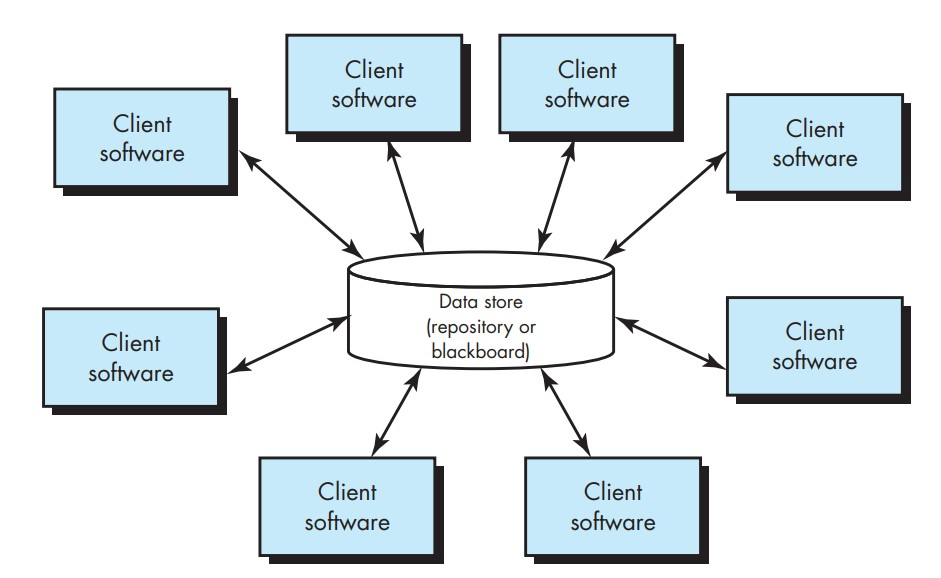
\includegraphics[scale=.45]{img/m2_36.jpg}
		\caption{Data-centered 
			architecture }
	\end{figure}
	
\end{frame}
\begin{frame}{ARCHITECTURAL STYLES}
	\textbf{Data-flow architectures.}
	\begin{itemize}
		\item \textbf{Shows the flow of input data}, its \textbf{computational components}
		and \textbf{output data}
		\item Structure is \textbf{also called pipe and Filter}
		\item \textbf{Pipe }provides path for \textbf{flow of data}
		\item \textbf{Filters manipulate data} and work independent of its
		neighboring filter
		\item If data flow degenerates into a single line of transform, it is
		termed as batch sequential.
	\end{itemize}	
\end{frame}
\begin{frame}{ARCHITECTURAL STYLES}
	\textbf{Data-flow architectures.}
	\begin{figure}
		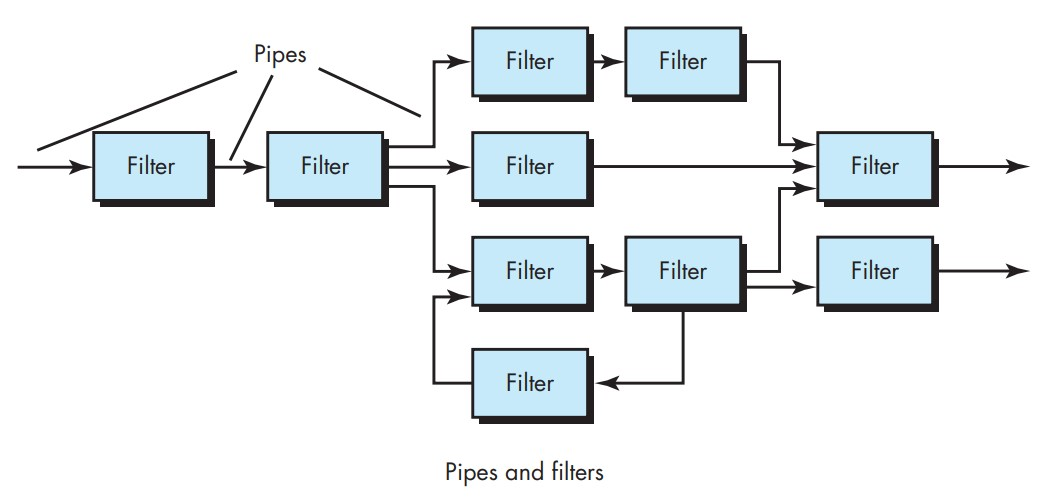
\includegraphics[scale=.45]{img/m2_37.jpg}
		\caption{Data-flow 
			architecture }
	\end{figure}
	
\end{frame}
\begin{frame}{ARCHITECTURAL STYLES}
	\textbf{Call and return architectures.}
	\begin{itemize}
		\item This architectural style enables you 
		to achieve a program structure that is relatively easy to modify and 
		scale. 
		\item A number of sub styles exist within this category:
		\begin{itemize}
			\item \textbf{Main program/subprogram architectures:}This classic 
			program structure decomposes function into a control 
			hierarchy where a “main” program invokes a number of 
			program components that in turn may invoke still other 
			components. 
			\item \textbf{Remote procedure call architectures. :}The components of a main program/subprogram architecture are distributed across 
			multiple computers on a network.

			
		\end{itemize}
	\end{itemize}
\end{frame}
\begin{frame}{ARCHITECTURAL STYLES}
	\textbf{Call and return architectures.}
	\begin{figure}
		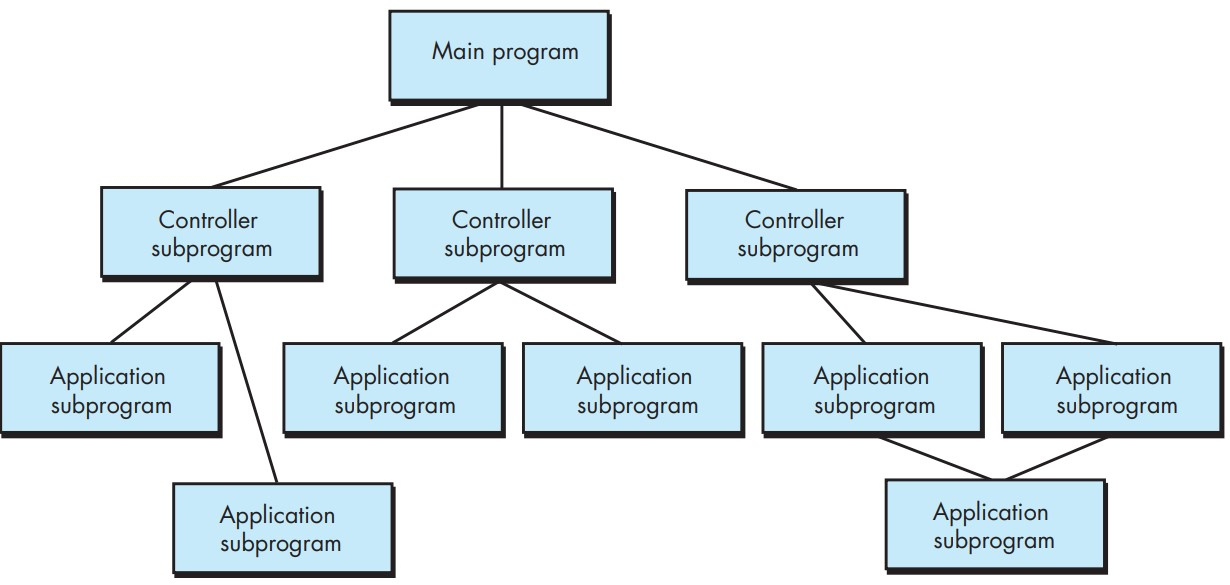
\includegraphics[scale=.45]{img/m2_38.jpg}
		\caption{Main program/
			subprogram 
			architecture }
	\end{figure}
	
\end{frame}
\begin{frame}{ARCHITECTURAL STYLES}
	\textbf{Object-Oriented Architectures. .}
\begin{itemize}
	\item The components of a system \textbf{encapsulate data and the 
		operations} that must be applied to manipulate the data.
	\item \textbf{Communication and coordination }
	between components are accomplished \textbf{via message passing.}
\end{itemize}
\end{frame}
\begin{frame}{ARCHITECTURAL STYLES}
	\textbf{Layered architectures. }
	\begin{itemize}
		\item A number of different layers are defined
		\item Inner Layer( interface with OS)
		\item Intermediate Layer Utility services and application function)
		\item Outer Layer (User interface)
	\end{itemize}
\end{frame}

\begin{frame}{ARCHITECTURAL STYLES}
	\textbf{Layered architectures. }
\begin{figure}
	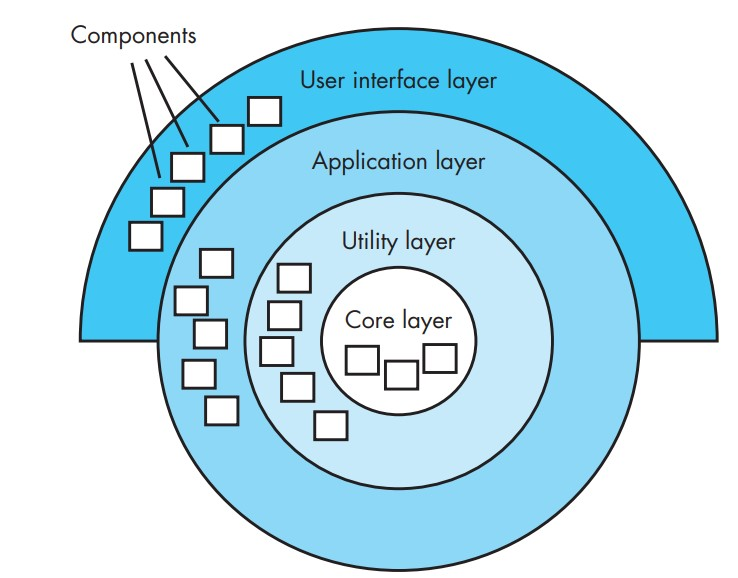
\includegraphics[scale=.45]{img/m2_39.jpg}
	\caption{Layered 
		architecture }
\end{figure}
\end{frame}
\begin{frame}{ARCHITECTURAL CONSIDERATIONS}
	\textbf{ARCHITECTURAL CONSIDERATIONS}
	\begin{itemize}
		\item Before proceeding to the final plan of constructing the structure, the firm have to mull about various aesthetic aspects to get the desired product. These aspects are known as Architectural Considerations.
		\item the are various architectural considerations made are as follows:
		\begin{itemize}
		\item \textbf{Economy:} 
		
		\item \textbf{Visibility:} 
		\item \textbf{Symmetry:} 
		
		\item \textbf{Emergence:} 
		\item \textbf{Spacing:}
		\end{itemize}
	\end{itemize}
\end{frame}
\begin{frame}{ARCHITECTURAL CONSIDERATIONS}
	\textbf{ARCHITECTURAL CONSIDERATIONS}
		\begin{itemize}
			\item \textbf{Economy:} The architecture prepared must be economically feasible. It should not contain unnecessary structures, which may result in the increase of dead load and loss of finances in the construction.
			
			\item \textbf{Visibility:} The drawings and the design layouts prepared by the design engineer should be elucidated to the workers on site, in order to provide visibility of the final product. They should be made to ensure the ease of understanding of design.
			
			\item \textbf{Symmetry:} It is necessary to ensure that the consistency of the product, with the presented layout of the design as maintained by the design engineer.
			
			\item \textbf{Emergence:} The idea of the structure to be constructed must be very clear from the drawings prepared.
			\item \textbf{Spacing:}  Separation of concerns in a design without introducing hidden dependencies is 
			a desirable design concept that is sometimes referred to as spacing. Sufficient spacing leads 
			to modular designs, but too much spacing leads to fragmentation and loss of visibility.
		\end{itemize}
\end{frame}
\begin{frame}{ARCHITECTURAL DESIGN}
	\textbf{ARCHITECTURAL DESIGN}
	\begin{itemize}
		\item The design should define the external entities (other systems, devices, people) that the software 
		interacts with and the nature of the interaction
		\item The three component of architectural design
		\begin{itemize}
			\item \textbf{Architectural context diagram:} model how
			software interacts with external entities
			\item \textbf{Archetypes:} are classes or patterns that represent an abstraction critical to the system
			\item \textbf{Architectural components} are derived from
			the application domain, the infrastructure, and	the interface
		\end{itemize}
	\end{itemize}
\end{frame}
\begin{frame}{ARCHITECTURAL DESIGN}
	\textbf{Representing the System in Context}
	\begin{itemize}
		\item At the architectural design level, a software architect uses an \textbf{architectural context diagram(ACD)} to model the manner in which 
		software interacts with entities external to its boundaries. 
		
		\begin{figure}
			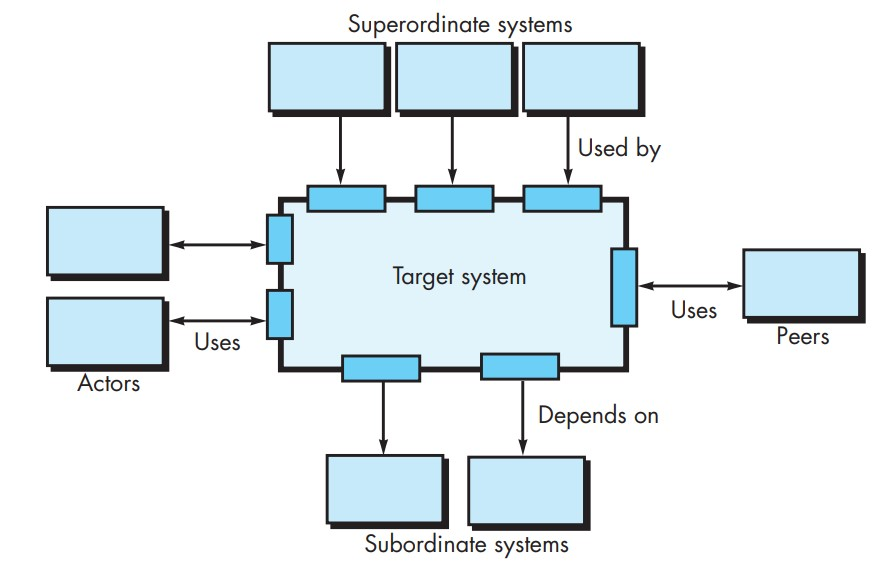
\includegraphics[scale=.45]{img/m2_40.jpg}
			\caption{Architectural context diagram}
		\end{figure}
		
	\end{itemize}
\end{frame}
\begin{frame}{ARCHITECTURAL DESIGN}
	\textbf{Representing the System in Context}
	
		\begin{figure}
			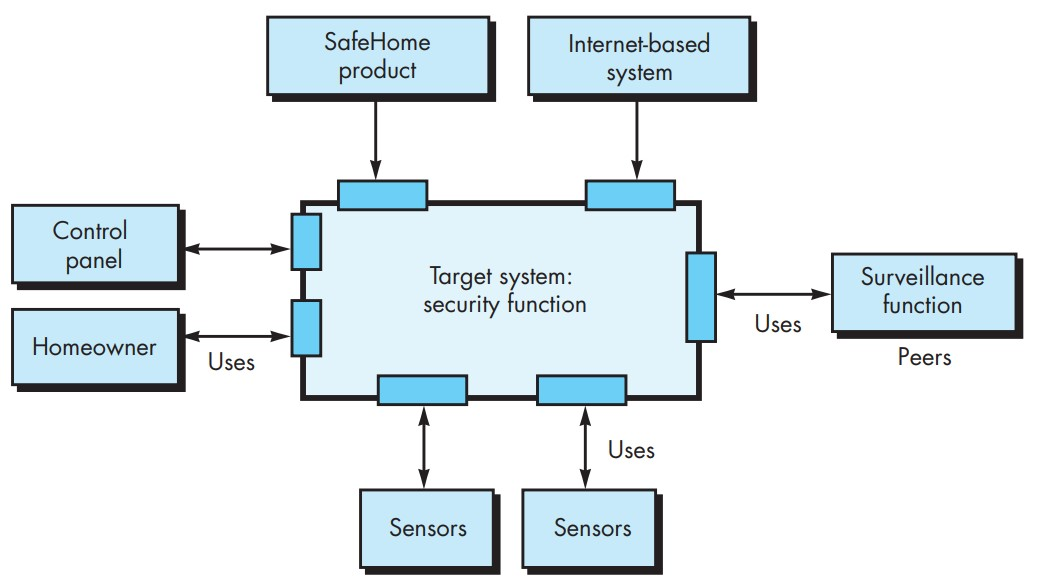
\includegraphics[scale=.45]{img/m2_41.jpg}
			\caption{Architectural 
				context 
				diagram for 
				the SafeHome
				security 
				function}
		\end{figure}
		

\end{frame}
\begin{frame}{ARCHITECTURAL DESIGN}
	\textbf{Representing the System in Context cont..}\\
	“Referring to the figure, systems that interoperate with
	the target system are represented as
	\begin{itemize}
		\item \textbf{Superordinate systems:} those systems that use the
		target system as part of some higher-level processing
		scheme.
			\item \textbf{Subordinate systems:} those systems that are used
		by the target system and provide data or processing
		that are necessary to complete target system
		functionality.
	\item \textbf{Peer-level systems:}those systems that interact on a
		peer-to-peer basis (i.e., information is either produced
		or consumed by the peers and the target system.
	\item \textbf{Actors:} entities (people, devices) that interact with
		the target system by producing or consuming
		information that is necessary for requisite processing.
	\end{itemize}
\end{frame}
\begin{frame}{ARCHITECTURAL DESIGN}
	\textbf{ Defining Archetypes}
	\begin{itemize}
		\item An archetype is a \textbf{class or pattern} that\textbf{ represents a
			core abstraction} that is critical to the design of an
		architecture for the target system.
		\item The following archetypes can be used in home security
		system architecture :
		\begin{itemize}
			\item Node.
			\item Detector.
			\item Indicator.
			\item Controller.
		\end{itemize}
	\end{itemize}
\end{frame}

\begin{frame}{ARCHITECTURAL DESIGN}
\textbf{ Defining Archetypes}
	
	\begin{figure}
		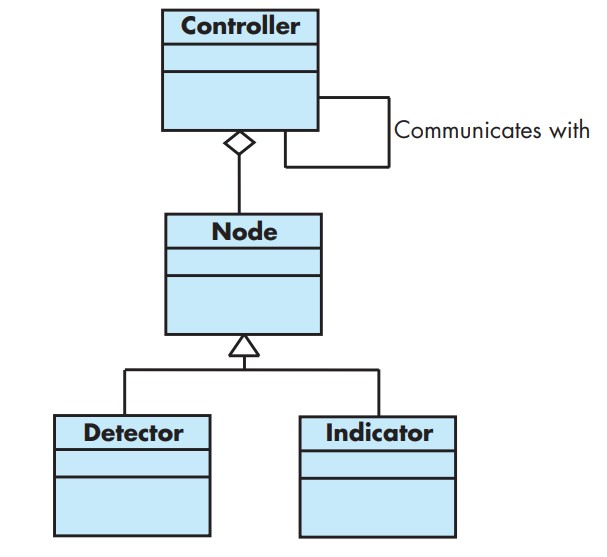
\includegraphics[scale=.45]{img/m2_42.jpg}
		\caption{UML relationships for 
			SafeHome
			security 
			function 
			archetypes }
	\end{figure}
	
	
\end{frame}
\begin{frame}{ARCHITECTURAL DESIGN}
	\textbf{ Defining Archetypes}
	\begin{itemize}
		\item \textbf{Node.} Represents a cohesive collection of input and output 	elements of the home security function. 
	\begin{itemize}
		\item For example a node might be comprised of (1) various sensors and (2) a variety of alarm (output) indicators.

	\end{itemize}
		\item \textbf{Detector. }An abstraction that encompasses all sensing 
		equipment that feeds information into the target system.
		\item \textbf{Indicator}. An abstraction that represents all mechanisms 
		(e.g., alarm siren,flashing lights, bell) for indicating that 
		an alarm condition is occurring.
	\item  \textbf{Controller}. An abstraction that depicts the mechanism 
		that allows the arming or disarming of a node. If controllers reside on a network, they have the ability to communicate with one another.
	\end{itemize}
	
	
\end{frame}
\begin{frame}{ARCHITECTURAL DESIGN}
	\textbf{Refining the Architecture into Components}
	\begin{itemize}
		\item As the software architecture is refined into component.
		\item The components 
		are derived from analysis class within application domain.
		\item Also, many infrastructure components are derived apart from 
		application domain components. Eg. Memory management 
		component.
		\item For eg, Based on the functionality, the following components are 
		derived from SafeHome home security function: 
		\begin{itemize}
			\item External communication management—coordinates 
			communication of the security function with external entities 
			such as other Internet-based systems and external alarm 
			notification.
		\item Control panel processing—manages all control panel functionality.
		\item  Detector management—coordinates access to all detectors attached 
			to the system.
			\item Alarm processing—verifies and acts on all alarm conditions.

		\end{itemize}
	\item Each of these top-level components would have to be elaborated 
	iteratively and then positioned within the overall architecture.
	\end{itemize}
\end{frame}
\begin{frame}{ARCHITECTURAL DESIGN}
%	\textbf{Refining the Architecture into Components}
	\begin{figure}
		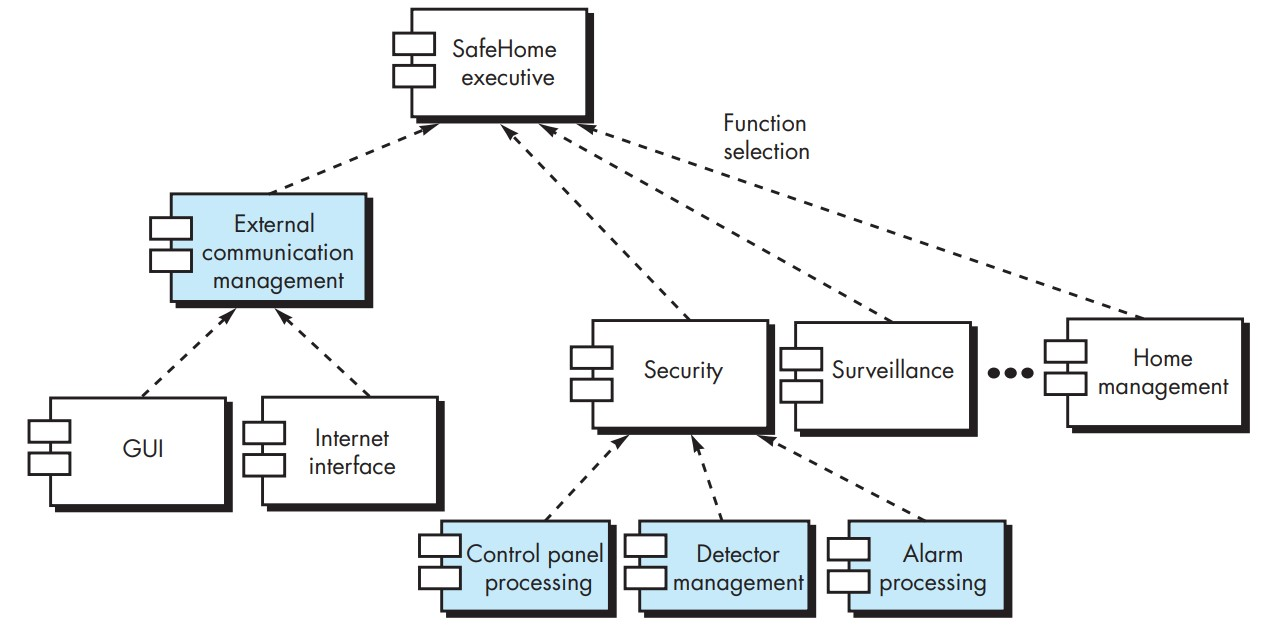
\includegraphics[scale=.45]{img/m2_44.jpg}
		\caption{Overall architectural structure for SafeHome with top-level components}
	\end{figure}
\end{frame}
\begin{frame}{ARCHITECTURAL DESIGN}
\textbf{Describing Instantiations of the System}
	\begin{itemize}
		\item The architectural design that has been modeled to this point is still relatively high level. 
		\item The context of the system has been represented 
		\item Archetypes that indicate the important abstractions within the problem domain have been defined, 
		\item The overall structure of the system is apparent, and the major software components have been identified. 
		\item However, further refinement is still necessary. 
		\item To accomplish this, an actual instantiation of the architecture is developed.It means, again it simplify by more details. 
	\end{itemize}
\end{frame}
\begin{frame}{ARCHITECTURAL DESIGN}
	\textbf{Describing Instantiations of the System}
		\begin{figure}
		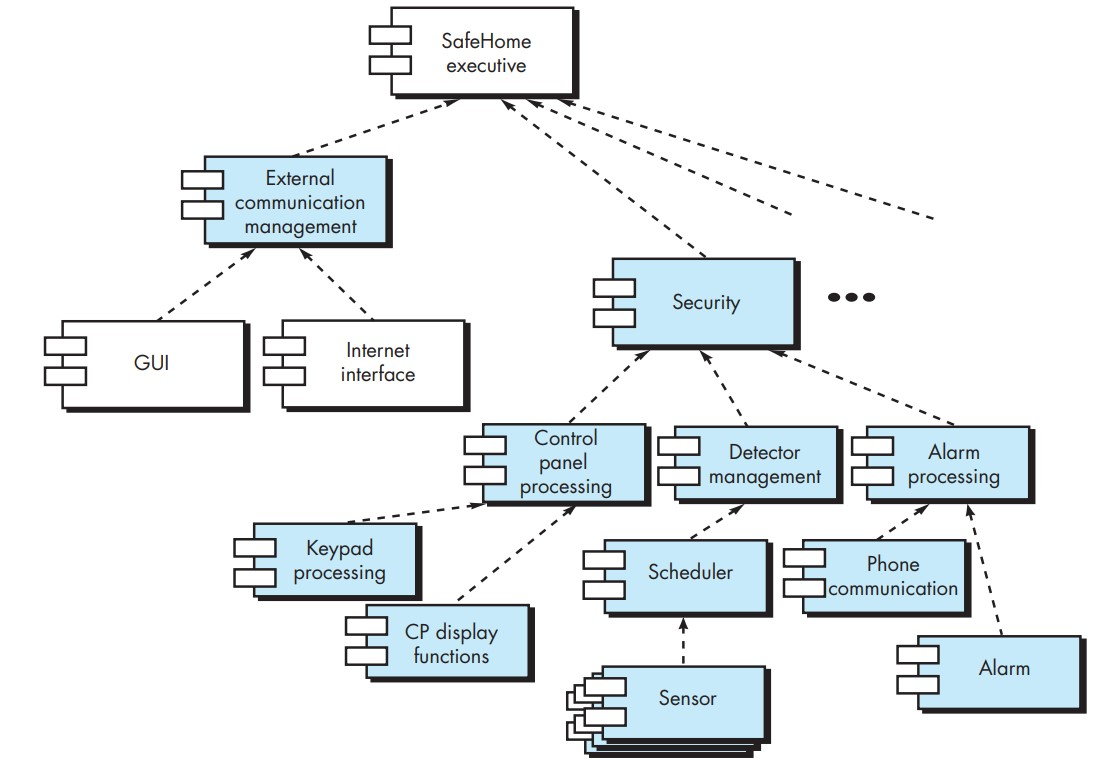
\includegraphics[scale=.45]{img/m2_45.jpg}
		\caption{An instantiation of the security function with component elaboration}
	\end{figure}
\end{frame}

\begin{frame}{ARCHITECTURAL DESIGN}
	\textbf{Architectural Design for Web Apps}
	\begin{itemize}
		\item WebApps are client-server applications
		\item structured using multilayered 
		architectures
		 including \begin{itemize}
		 	\item a user interface or view layer, 
		 	\item a controller layer which directs the 
		 	flow of information to and from the client browser based on a set of business rules, and 
		 	\item a 
		 	content or model layer that may also contain the business rules for the WebApp.

		 \end{itemize}
	\end{itemize}
\end{frame}

\begin{frame}{ARCHITECTURAL DESIGN}
	\textbf{Architectural Design for Mobile Apps}
	\begin{itemize}
		\item Mobile apps are typically structured using multilayered architectures, including a user 
		interface layer, a business layer, and a data layer. 
		\item With mobile apps you have the choice of 
		building a thin Web-based client or a rich client. With a thin client, only the user interface 
		resides on the mobile device, whereas the business and data layers reside on a server. With 
		a rich client all three layers may reside on the mobile device itself.

		\end{itemize}
\end{frame}
\section{ Component level design }
\begin{frame}{Component level design }
	\textbf{Component level design }
	\begin{itemize}
		\item A software component is a modular building block for the computer software.
		\item Component is defined as a modular, deployable and replaceable part of the system which encloses the implementation and exposes a set of interfaces.
	\end{itemize}
\end{frame}
\begin{frame}{Component level design }
	\textbf{The components has different views as follows:}
	\begin{itemize}
		\item An object-oriented view
		\item The traditional view
		\item The Process related view
	\end{itemize}
\end{frame}
\begin{frame}{Component level design }
	\textbf{An object-oriented view:}
	\begin{itemize}
		\item An object-oriented view is a set of collaborating classes.
		\item The class inside a component is completely elaborated and it \textbf{consists of all the attributes and operations} which are applicable to its implementation.
		\item To achieve object-oriented design it elaborates analysis classes and the infrastructure classes.
	\end{itemize}
\end{frame}
\begin{frame}{Component level design }
	\textbf{An object-oriented view:}
	\begin{figure}
	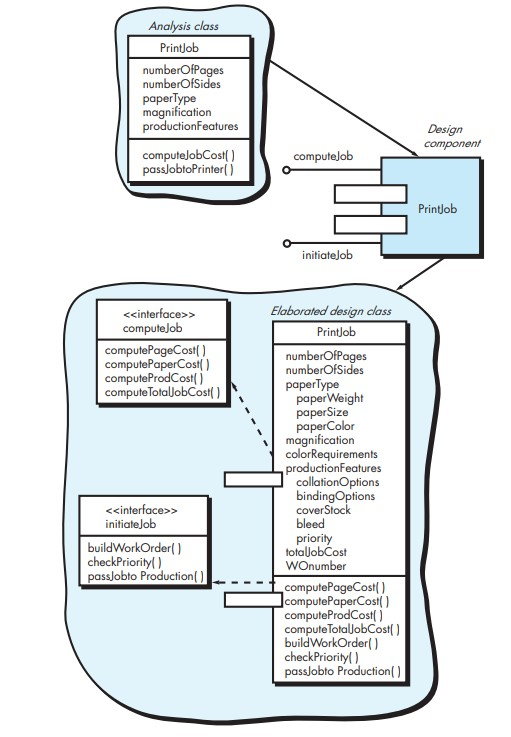
\includegraphics[scale=.46]{img/m2_46.jpg}
	\caption{elaboration of design component
	}
\end{figure}
\end{frame}

	

\begin{frame}{Component level design }
	\textbf{The traditional view}
	\begin{itemize}
		\item In the context of traditional software engineering, a component is a \textbf{functional element of a program }that incorporates 
		\begin{itemize}
			\item \textbf{Processing logic}, 
			\item \textbf{The internal data structures} that are required to implement the processing logic, 
			\item\textbf{ An interface} that enables the component to be invoked and data to be passed to it. 
		\end{itemize}
	\item A traditional component, also called a module,
		\item It resides in the software and serves\textbf{ three important roles} 
		\begin{itemize}
			\item \textbf{Control component}
			\begin{itemize}
				\item A control component coordinate is an invocation of all other problem domain components.
			\end{itemize}
			\item  \textbf{Problem domain component }
				\begin{itemize}
				\item A problem domain component implements a complete function which is needed by the customer.
			\end{itemize}
			\item \textbf{Infrastructure component}.
				\begin{itemize}
				\item An infrastructure component is responsible for function which support the processing needed in the problem domain.
			\end{itemize}
		\end{itemize}
	\end{itemize}
\end{frame}


\begin{frame}{Component level design }
	\begin{figure}
	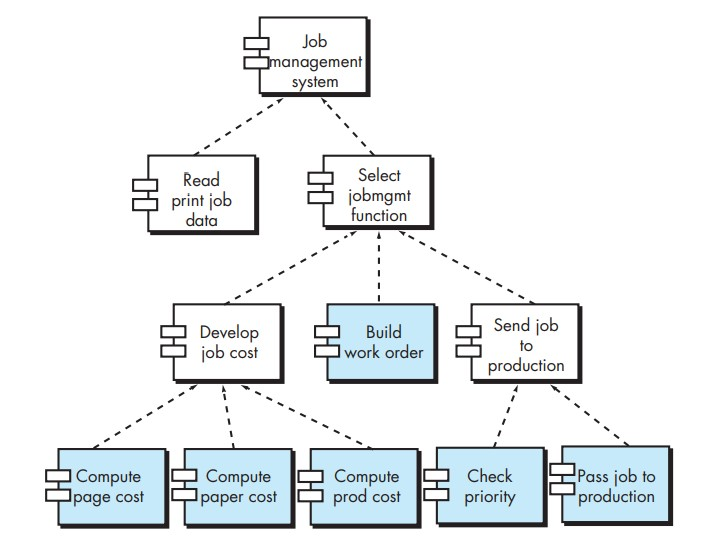
\includegraphics[scale=.46]{img/m2_47.jpg}
	\caption{Structure chart for a traditional system}
\end{figure}
\end{frame}


\begin{frame}{Component level design }
	\textbf{A Process-Related View}
	\begin{itemize}
		\item This view highlights the building system out of existing components.
		\item The design patterns are selected from a catalog and used to populate the architecture.
	\end{itemize}
\end{frame}
\begin{frame}{Component level design }
	\textbf{Class-based design components}
	\begin{itemize}
		\item The principles for class-based design component are as follows:
		\begin{enumerate}
			\item Open Closed Principle (OCP)
			\item The Liskov Substitution Principle (LSP)
			\item Dependency Inversion Principle (DIP)
			\item The Interface Segregation Principle (ISP)
			\item The Release Reuse Equivalency Principle (REP)
			\item The common closure principle (CCP)
			\item The Common Reuse Principle (CRP)
		\end{enumerate}
	\end{itemize}
\end{frame}
\begin{frame}{Component level design }
	\textbf{Open Closed Principle (OCP)}
	\begin{itemize}
		\item \textbf{“A module [component] 
			should be open for extension but closed for modification”}
		\item Should specify the component in a way that allows it to be extended (within 
		the functional domain that it addresses) without the need to make internal (code 
		or logic-level) modifications to the component itself. 
	
	\end{itemize}
	\begin{figure}
	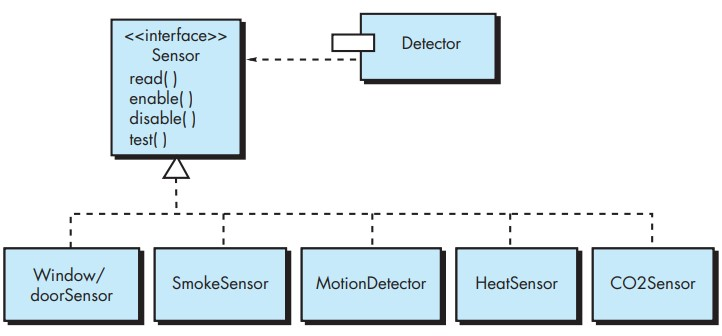
\includegraphics[scale=.46]{img/m2_48.jpg}
	\caption{Following the OCP}
\end{figure}

\end{frame}
\begin{frame}{Component level design }
	\textbf{The Liskov Substitution Principle (LSP)}
	\begin{itemize}
		\item \textbf{“Subclasses should be 
			substitutable for their base classes”.} 
		\item This design principle suggests that a component that uses a base class should 
		continue to function properly if a class derived from the base class is passed
		to the component instead
		\item In the context, a “contract” is a pre-condition that must be true before the 
		component uses a base class and a post-condition that should be true after 
		the component uses a base class. When you create derived classes, be sure
		they conform to the pre- and post-conditions
		
	\end{itemize}	
\end{frame}
\begin{frame}{Component level design }
	\textbf{Dependency Inversion Principle (DIP)}
		\begin{itemize}
			\item \textbf{“Depend on abstractions. Do not dependon concretions”. }
			\item The more a component depends on 
			other concrete components, the more difficult it will be to extend
		\end{itemize}
\end{frame}
\begin{frame}{Component level design }
	\textbf{The Interface Segregation (Separation) Principle (ISP).}
	\begin{itemize}
		\item \textbf{“Many client-specific interfaces are better than one general purpose interface. "}
		\item There are many instances in which multiple client components use the 
		operations provided by a server class.
		\item Should create a specialized interface to serve each major category of 
		clients. Only those operations that are relevant to a particular category of 
		clients should be specified in the interface for that client. If multiple clients 
		require the same operations, it should be specified in each of specialized
		interfaces.
	\end{itemize}
\end{frame}

\begin{frame}{Component level design }
	\textbf{The Release Reuse Equivalency Principle (REP)}
	\begin{itemize}
		\item \textbf{“The granule of reuse is the granule of release”}
		\item When classes or components are designed for reuse, an implicit contract is 
		established between the developer of the reusable entity and the people who 
		will use it.
		\item The developer commits to establish a release control system that supports
		and maintains older versions of the entity while theusers slowly upgrade to
		the most current version. 
	\end{itemize}
\end{frame}

\begin{frame}{Component level design }
	\textbf{The Common Closure Principle (CCP). }
	\begin{itemize}
		\item \textbf{“Classes that change together belong together.” }
		\item That is, when classes are packaged as part of a design, they should address 
		the same functional or behavioural area.
	\item When some characteristic of that area must change, it is likely that only
		those classes within the package willrequire modification. Thisleadstomore
		effective change control and release management
		
	\end{itemize}
\end{frame}
\begin{frame}{Component level design }
	\textbf{The Common Reuse Principle (CRP).}
	\begin{itemize}
		\item \textbf{“Classes that aren’t reused together should not be grouped together”  }
		\item  When one or more classes with a package changes, the release number of 
		the package changes.
		\item All other classes or packages that rely on the package that has been changed 
		must now update to the most recent release of the package and be tested to 
		ensure that the new release operated without incident.
		\item If classes are not grouped cohesively, it is possible that a class with no 
		relationship to other classes within a package is changed. This will precipitate
		unnecessary integration and testing.
		\item For this reason, only classes that are reused together should be included
		within a package.

	\end{itemize}
\end{frame}
\begin{frame}{Component level design }
	\textbf{Component-Level Design Guidelines}
	\begin{itemize}
		\item In addition to the principles , a set of pragmatic (Practical) design guidelines can be applied as component-level design proceeds. 
		\item These guidelines apply to 
		\begin{itemize}
			\item Components, 
			\item Interfaces 
			\item Dependencies and inheritance 
		\end{itemize}
	\end{itemize}
\end{frame}
\begin{frame}{Component level design }
	%\textbf{Component-Level Design Guidelines}\\
	\textbf{Components }
	\begin{itemize}
		\item Naming conventions should be established for components that are specified as part of the architectural model and then refined and elaborated as part of the component-level model
	\end{itemize}
	\textbf{Interfaces }
	\begin{itemize}
		\item Interfaces provide important information about communication and collaboration.
	\end{itemize}
	\textbf{Dependencies and Inheritance }
	\begin{itemize}
		\item For improved readability,
		\item it is a good idea to model dependencies from left to right and inheritance from bottom (derived classes) to top (base classes).
	\end{itemize}
\end{frame}
\begin{frame}{Component level design }
	\textbf{Cohesion}
	\begin{itemize}
		\item Implies that a component or class encapsulates only attributes and operations that are closely related to one another and to the class or component itself.
		\item Levels of cohesion OR different types of cohesion
		\begin{itemize}
			\item Functional
			\item Layer
			\item Communicational
		\end{itemize}
	\end{itemize}
\end{frame}
\begin{frame}{Component level design}
	\textbf{Functional}
	\begin{itemize}
		\item Exhibited primarily by operations, this level of cohesion occurs when a module performs one and only one computation and then returns a result.
	\end{itemize}
	\textbf{Layer} 
	\begin{itemize}
		\item Exhibited by packages, components, and classes, this type of cohesion occurs when a higher layer accesses the services of a lower layer, but lower layers do not access higher layers.
	\end{itemize}   
	\textbf{Communicational}
	\begin{itemize}
		\item All operations that access the same data are defined within one class. In general, such classes focus solely on the data in question, accessing and storing it.
	\end{itemize}
\end{frame}
\begin{frame}{Component level design}
\textbf{Coupling}
\begin{itemize}
	\item Coupling is a qualitative measure of the degree to which classes are 
	connected to one another. 
	\item As classes (and components) become more 
	interdependent, coupling increases.
	\item  An important objective in 
	component-level design is to \textbf{keep coupling as low as is possible}.

\end{itemize}
\end{frame}
\begin{frame}{Component level design}
	\textbf{Types of Coupling}
	\begin{itemize}
		\item \textbf{Content Coupling:}
		\begin{itemize}
			\item It occurs when one component “surreptitiously modifies data that is internal to another 
			component”. 
			\item It violates information hiding.
		\end{itemize}
         	\item \textbf{Control coupling:}
         	\begin{itemize}
         		\item Occurs when operation A() invokes operation B() and 
         		passes a control flag to
         		B.
         		\item  The control flag then “directs” logical flow within B. The problem 
         		with this form of coupling is that an unrelated change in B can result 
         		in the necessity to change the meaning of the control flag that A 
         		passes. If this is overlooked, an error will result.
         	\end{itemize}
         \item \textbf{External coupling }
         \begin{itemize}
         	\item Occurs when a component communicates or 
         	collaborates with infrastructure components (e.g., operating system 
         	functions, database capability, tele-communication functions). 
         	\item Although this type of coupling is necessary, it should be limited to a 
         	small number of components or classes within a system.
         \end{itemize}
	\end{itemize}
\end{frame}
\begin{frame}{Component level design}
	\textbf{CONDUCTING COMPONENT-LEVEL DESIGN}
	\begin{itemize}
		\item The following \textbf{steps represent a typical task set for component-level design}, when 
		it is applied for an object-oriented system.
	\begin{enumerate}
		\item Identify Design Classes in Problem Domain
		\item Identify Infrastructure Design Classes
		\item Elaborate Design Classes
		\item Describe Persistent Data Sources
		\item Elaborate Behavioral Representations
		\item Elaborate Deployment Diagrams
		\item Refactor Design And Consider Alternatives
	\end{enumerate}
	\end{itemize}
\end{frame}

\begin{frame}{Component level design}
%	\textbf{CONDUCTING COMPONENT-LEVEL DESIGN}
	\begin{itemize}
		\item[1] Identify all design classes that correspond to the problem domain.
		\begin{itemize}
			\item Using
			the requirements and architectural model, each analysis class and architectural
			component is elaborated
		\end{itemize}
		\item[2] Identify all design classes that correspond to the infrastructure domain.
		\begin{itemize}
			
			\item These classes are not described in the requirements model and are often missing
			from the architecture model, but they must be described at this point. Classes and 
			components in this category include \textbf{GUI components} (often available as reusable components), \textbf{operating system components}, and \textbf{object and data management
				components}.
			
		\end{itemize}
		\item[3] Elaborate all design classes that are not acquired as reusable components.
		\begin{itemize}
			\item Elaboration requires that \textbf{all interfaces, attributes, and operations necessary to
				implement the class be described in detail}. Design heuristics (e.g., component
			cohesion and coupling) must be considered as this task is conducted.

		\end{itemize}
	\end{itemize}
\end{frame}


\begin{frame}{Component level design}
	%\textbf{CONDUCTING COMPONENT-LEVEL DESIGN}
	\begin{itemize}
		\item[3a] Specify message details when classes or components collaborate.
		\begin{itemize}
			\item  The 	requirements model makes use of a collaboration diagram to show how analysis classes
			collaborate with one another. Messages that are passed between objects within a
			system.
		\end{itemize}
	\end{itemize}	

	\begin{figure}
	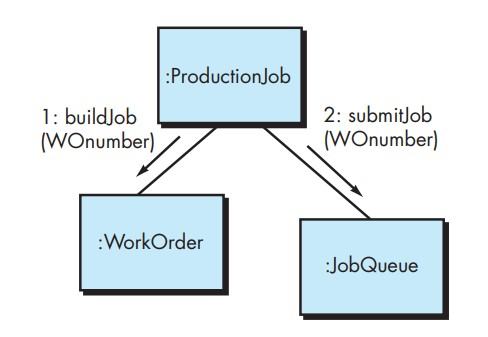
\includegraphics[scale=.46]{img/m2_49.jpg}
	\caption{Collaboration 
		diagram with 
		messaging}
\end{figure}

\end{frame}




\begin{frame}{Component level design}
%	\textbf{CONDUCTING COMPONENT-LEVEL DESIGN}
	\begin{itemize}
		\item[3b] Identify appropriate interfaces for each component.
		\begin{itemize}
			\item Within the context of 
			component-level design, a UML interface is “a group of externally visible (i.e.,
			public) operations. The interface contains no internal structure, it has no attributes,no 
			associations. “.

		\end{itemize}
	
	\end{itemize}	
%	\begin{figure}
%	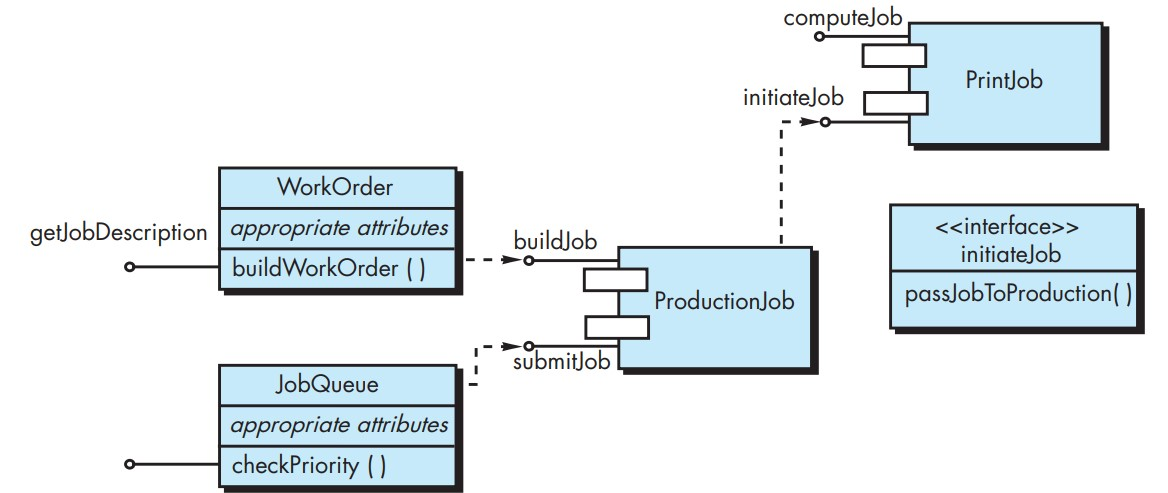
\includegraphics[scale=.46]{img/m2_50.jpg}
%	\caption{Refactoring interfaces and class definitions for PrintJob }
%\end{figure}
\end{frame}



\begin{frame}{Component level design}
%	\textbf{CONDUCTING COMPONENT-LEVEL DESIGN}
	\begin{itemize}
		
		\item[3c] Elaborate attributes and define data types and data structures required to 
		implement them. 
		\begin{itemize}
			\item In general, data structures and types used to define attributes are
			defined within the context of the programming language that is to be used for 
			implementation.
		\end{itemize}
	\end{itemize}	

\end{frame}


\begin{frame}{Component level design}
%	\textbf{CONDUCTING COMPONENT-LEVEL DESIGN}
	\begin{itemize}
		\item[3d] Describe processing flow within each operation in detail. 
		\begin{itemize}
			\item This may be
			accomplished using a programming language-based pseudo code or with a UML
			activity diagram. Each software component is elaborated through a number of
			iterations that apply the stepwise refinement concept.
			
		\end{itemize}
	
	\end{itemize}	


\begin{figure}
	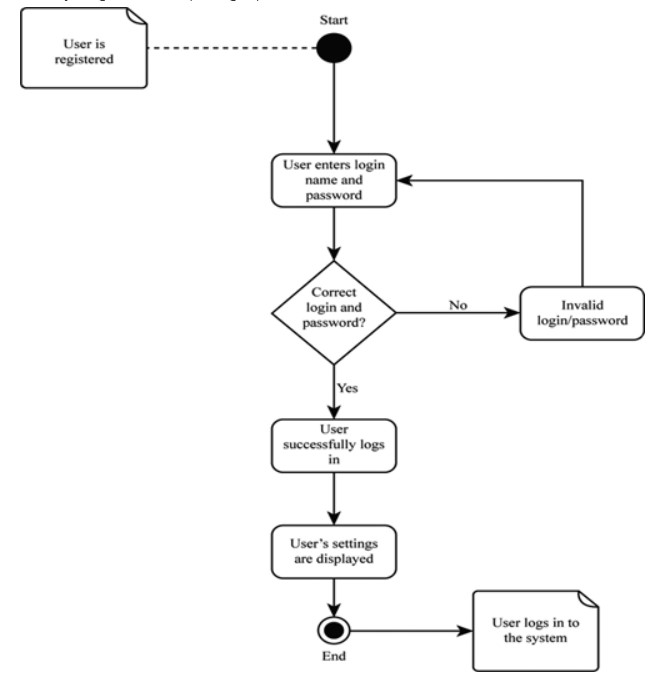
\includegraphics[scale=.33]{img/m2_51.jpg}
	\caption{UML activity 
		diagram for 
		simple login procedure: }
\end{figure}
\end{frame}
\begin{frame}{Component level design}
%	\textbf{CONDUCTING COMPONENT-LEVEL DESIGN}
	\begin{itemize}
		\item[4] Describe persistent data sources (databases and files) and identify the
		classes required to manage them. 
		\begin{itemize}
			\item The persistent data sources are described (databases and files) and the classes required to 
			manage them are identified.
		\end{itemize}
	\end{itemize}	
\end{frame}


\begin{frame}{Component level design}
	%	\textbf{CONDUCTING COMPONENT-LEVEL DESIGN}
	\begin{itemize}
		\item[5] Develop and elaborate behavioural representations for a class or
		component.
		\begin{itemize}
			\item It is sometimes necessary to model the behavior of a design class.
			\item The behavior of the system is elaborated using a state diagram to depict the transition of 
			states during work flow.
		\end{itemize}
	\end{itemize}	
	
	\begin{figure}
		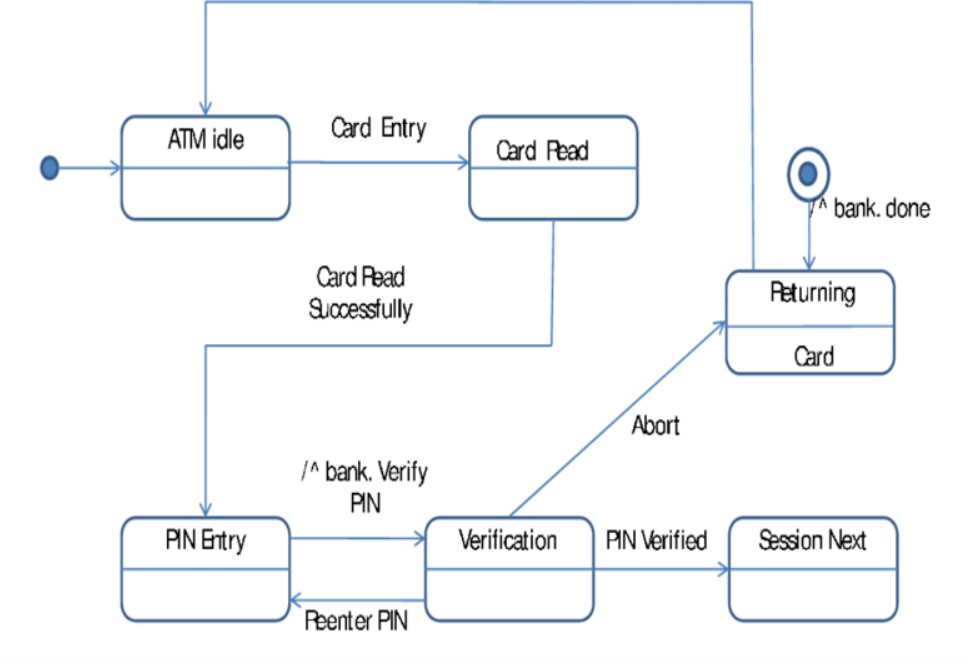
\includegraphics[scale=.35]{img/m2_52.jpg}
		\caption{Statechart 
			fragment for 
			Simple ATM Diagram }
	\end{figure}
\end{frame}

\begin{frame}{Component level design}
	%\textbf{CONDUCTING COMPONENT-LEVEL DESIGN}
	\begin{itemize}
		\item[6] Elaborate deployment diagrams to provide additional implementation
		detail. 
		\begin{itemize}
			\item Deployment diagrams are used as part of architectural design and are 
			represented in descriptor form. In this form, major system functions (often represented as subsystems) are represented within the context of the computing
			environment that will house them.
		\end{itemize}
	
	\end{itemize}	


\end{frame}

\begin{frame}{Component level design}
	%\textbf{CONDUCTING COMPONENT-LEVEL DESIGN}
	\begin{itemize}
		\item[7]Refactor every component-level design representation and always con- sider
		alternatives
		\begin{itemize}
			\item Design is an iterative process. The first component-level model we
			create will not be as complete,consistent, or accurate as the nth iteration you apply 
			to the model. It is essential to refactor as design work is conducted.
		\end{itemize}
	\end{itemize}	
\end{frame}


\begin{frame}{Component level design}
	\textbf{Component Level Design for WebApps}
	\begin{itemize}
		\item A WebApp component is 
		\begin{itemize}
			\item A well-defined cohesive (Interrelated) function that manipulates content or provides computational or data processing for an end user
			\item A cohesive package of content and functionality that provides the end user with some required capability. 
			\item Therefore, component-level design for WebApps often incorporates elements of 
			\begin{itemize}
				\item Content design 
				\item Functional design.
			\end{itemize}
		\end{itemize}
	\end{itemize}	
\end{frame}
\begin{frame}{Component level design}
	\textbf{Content Design at the Component Level }
	\begin{itemize}
		\item Content design at the component level focuses on content objects and the manner in which they may be packaged for presentation to a WebApp end user. 
		\item The formality of content design at the component level should be tuned to the characteristics of the WebApp to be built. 
		\item However, as the size and complexity (of the WebApp, content objects, and their interrelationships) grows, it may be necessary to organize content in a way that allows easier reference and design. 
		\item For example, consider a Web-based video surveillance capability within SafeHomeAssured.com. Among many capabilities, the user can select and control any of the cameras represented as part of a floor plan, require video-capture thumbnail images from all the cameras, and display streaming video from any one camera.
	\end{itemize}	
\end{frame}
\begin{frame}{Component level design}
	\textbf{Functional Design at the Component Level }
	\begin{itemize}
		\item Modern Web applications deliver increasingly sophisticated processing functions that 
		\begin{itemize}
			\item Perform localized processing to generate content and navigation capability in a dynamic fashion, 
			\item Provide computation or data processing capability that is appropriate for the WebApp’s business domain, 
		\item Provide sophisticated database query and access, 
			\item Establish data interfaces with external corporate systems. 
		\end{itemize}
	\end{itemize}	
\end{frame}
\end{document}